\documentclass{report}
\usepackage{multicol}
\usepackage[utf8]{inputenc}
\usepackage[T1]{fontenc}
\usepackage{lmodern}
\usepackage[francais]{babel}
\usepackage{graphicx}
\usepackage{dblfloatfix}
\usepackage{circuitikz}
\usepackage[squaren, Gray]{SIunits}
\usepackage{sistyle}
\usepackage[autolanguage]{numprint}
\usepackage{pgfplots}
\usepackage{wrapfig}
%\usepackage{lipsum}
\usepackage{eurosym}
\usepackage[]{geometry}
\usepackage{fullpage}
\usepackage{hyperref}
\usepackage{caption}
\newcommand{\HRule}{\rule{\linewidth}{0.5mm}}
\usepackage{subcaption}
\usepackage{amsmath,amssymb,array}
\usepackage{url}
\usepackage{fancyhdr}
\usepackage{layout}
\newcommand\HUGE{\@setfontsize\Huge{38}{47}} 
\usepackage[version=3]{mhchem}
\usepackage{array} 
\usepackage{tikz}
\usepackage{here}
\usetikzlibrary{arrows,shapes,positioning}
\title{Synthèse du cours LAUCE1171 - Géomatériaux}
\author{Geoffroy Jacquet}
\date{ }
\begin{document}
\maketitle
\tableofcontents

\paragraph*{Remarque} Cette synthèse est divisée en deux parties, suivant le schéma du cours magistral. Cependant, certaines notions se recoupent dans les deux parties et ne sont donc expliquées qu'une seule fois (notamment la formation, classification des roches/sols).

\part{}

\chapter{Formation, nature et caractéristiques des sols}
\label{sols}

\section{Minéraux, roches et sols}
Il est important de bien distinguer trois termes : les minéraux, les roches et les sols. 
\paragraph*{Minéraux} Un minéral est une espèce chimique naturelle se présentant le plus souvent sous la forme d'un solide cristallin. La classification des minéraux est basée selon leur caractéristiques chimiques et cristallographiques.
\paragraph*{Roches} Ce sont des ensembles formés d'un ou plusieurs minéraux et se répartissent en trois grandes catégories : magmatiques (ou ignées), sédimentaires et métamorphiques.
\paragraph*{Sols} Les sols sont des formations naturelles de surface, meubles, résultant de la transformation, au contact de l'atmosphère, de la roche mère sous-jacente, sous l'influence de processus chimiques, physiques et biologiques. C'est un agrégat de particules solides entre lesquelles les espaces sont occupés par du gaz ou du liquide.

\subsection{Roches ignées}
Celles-ci proviennent directement de la solidification du magma (matière minérale en fusion) et peuvent être soit \textit{intrusives} (solidification en profondeur) soit \textit{extrusives} ou \textit{effusives} (solidification en surface). Dans le cas des roches intrusives (resp. extrusives), la vitesse de refroidissement est lente (resp. rapide) et il y aura formation de gros (resp. petis) cristaux. Les roches intrusives ont donc une texture rugueuse, et tous les grains sont identifiables, on dit qu'ils ont une texture phanéritique. Les roches intrusives ont une texture aphanitique (on ne voit pas les grains mais on les sent) ou vitreuse (grains indiscernables au toucher et à l'oeil nu) et parfois porphyrique, entre phanéritique et aphanitique.
\\
On distingue aussi deux type de roches ignées selon leur pH. Les roches acides (resp. basiques) proviennent de magmas acides (resp. basiques), sont riches en silicium (resp. fer et magnésium), ont une teinte claire (resp. foncée). Les magmas acides (resp. basiques) proviennent de la fusion de la croûte continentale (resp. océanique).

\subsection{Roches sédimentaires}
Elles se forment en surface (elles sont exogènes). Elles proviennent de transformation de sédiments en roches consolidées. Ces sédiments proviennent d'autres roches altérées ou de la faune et flore. La formation d'une roche sédimentaire commence par l'érosion, une destruction de roches existantes par divers acteurs physiques (vent,...) ou chimiques (dissolution de roche, minéraux,...). Les sédiments sont ensuite transporté (par le vent, cours d'eau,...) et finissent par se déposer. Vient ensuite le phénomène de diagénèse qui transforme les sédiment en roches. Les milieux sédimentaires sont des milieux d'accumulation des sédiments. Il existe des mileux continentaux (glaciers, déserts, lacs,... les sédiments sont transportés par le vent, le courant,... et se déposent lorsque l'agent n'a plus assez d'énergie que pour les transporter) et des mileux marins (plateau continental, talus continental et plaine abyssale).
Les principales roches sédimentaires sont :
\paragraph*{Roches détritiques} Formées à partir de roches préexistantes, composées de morceaux de roches et minéraux. 
\paragraph*{Roches carbonatées} Elles sont formées principalement de calcite et d'aragonite (\ce{CaCO3}) ou d'aragonite (\ce{MgCO3}).
\paragraph*{Roches siliceuses} Formées d'au moins 50\% de silice (\ce{SiO2}) d'origine chimique, biologique ou biochimique et provient de la dissolution d'organismes siliceux ou de roche.

\subsection{Roches métamorphiques}
Elles proviennent d'une transformation de roche existante suite à une augmentation de température ou de pression.
Cette transformation peut survenir au contact de magma (haute température, basse pression), suite à un enfouissement à grande profondeur (basse température, haute pression) ou encore suite à des plissements tectoniques (moyenne température et pression).
\paragraph*{Métamorphisme régional} Affecte des roches sur une vaste étendue. Recristallisation en minéraux de plus en plsu gros. Apparition d'une structure feuilletée suivant les plans d'applatissement (foliation).
\paragraph*{Métamorphisme de contact} Survient au contact de magma et se produit entre quelques mètres et quelques dizaines de mètres autour d'une poche de magma.
\paragraph*{Ultramétamorphisme} Suite à un enfouissement en profondeur, transformation en magma de certaines roches, d'autres restent solides.


\section{Cycle des roches}
La formation et la transformation des sols, minéraux et roches font partie du cycle géologique, comme montré à la figure~\ref{fig:cycle}.
\begin{figure}[ht]
\centering
\begin{subfigure}[h]{0.45\textwidth}
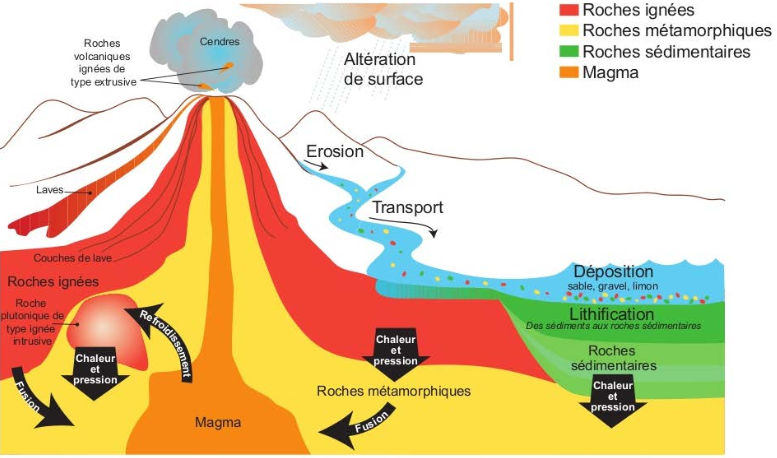
\includegraphics[scale=0.33]{Cycle_2.png}
\end{subfigure}
\qquad
\begin{subfigure}[h]{0.45\textwidth}
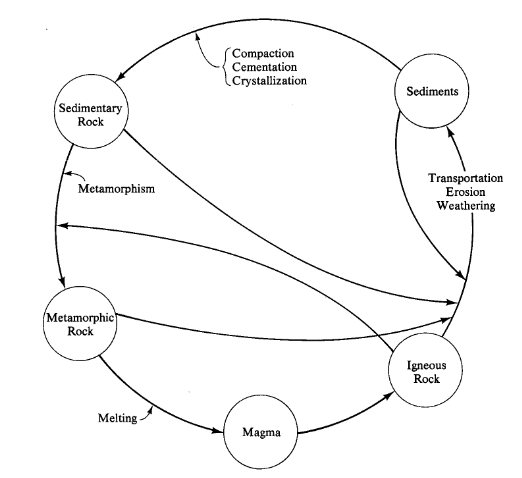
\includegraphics[scale=0.38]{Cycle_1.png}
\end{subfigure}
\caption{Cycle géologique}
\label{fig:cycle}
\end{figure}

Le cycle débute avec le magma qui se refroidit et se transforme en roches ignées. Ces roches sont dans un premier temps attaquées par l'oxygène, le \ce{CO2}, des changements de température,... et forment des sols résiduels. Des actions physiques ou chimiques sur ces roches peuvent mener, après transport à des dépôts sédimentaires qui peuvent à leur tour se consolider et former des roches sédimentaires. D'autres conditions supplémentaires (température, pression) mènent à la formation de roches métamorphiques. Les différentes roches peuvent être dégradées et rentrer dans le cycle à nouveau pour former une nouvelle roche ou bien former le sol si assez proche de la surface. Le sol est formé à partir de roche par décomposition physique ou chimique. L'ensemble de ces deux processus est appelé altération.

\subsection{Altération}
L'altération est la réduction en masse des roches, résultant d'une action physique où chimique.

\subsubsection{Altération mécanique}
L'altération se fait par :
\begin{itemize}
\item usure par frottement entre deux roches, abrasion par le vent, l'eau;
\item chocs entre éléments;
\item changements de température entrainant des cycles de contraintes alternés en traction/compression;
\item cycles de gel/dégel, l'eau dans les ouvertures de la roche gonfle suite au gel et peut créer des fissures. 
\end{itemize}
L'altération mécanique conduit principalement à la formation de sols grossiers (sable, gravier).

\subsubsection{Altération chimique}
L'altération se fait par : 
\begin{itemize}
\item oxydation : combinaison chimique de l'oxygène avec des minéraux;
\item hydratation : combinaison chimique de l'eau avec certains minéraux;
\item carbonation : combinaison chimique du dioxyde de carbone et de l'eau pour décomposer des minéraux (exemple : le calcaire);
\item interaction avec de la matière organique (végétation, bactéries,...).
\end{itemize}
L'altération chimique conduit principalement à la formation d'argiles et limons.

\subsection{Transport}
Le transport peut se faire de différentes manières :
\begin{itemize}
\item par gravité : glissements de terrains, coulées de boue,...;
\item par glaciers : ceux-ci bougent très lentement et écorchent la roche. Lors de la fonte, les matériaux sont accumulés sous la forme d'une \textit{moraine terminale};
\item par l'eau (pluie, cours d'eau,...) : la taille des éléments transportés varie en fonction de la vitesse de l'agent transporteur. Il y a trois parties : les particules les plus grossières glissent sur le fond, celles un peu plus petites roules sur le fond et les particules les plus fines restent en suspension dans l'eau;
\item par le vent : les éléments transportés sont fins et, contrairement à l'eau, le vent déplace les éléments d'un point bas à un point haut.
\end{itemize}

\section{Sable et argile}
Le sol peut se diviser en deux catégories : les grains fins (<\unit{0.06}{\milli\meter}), comprenant les argiles et limons, et grossiers (>\unit{0.06}{\milli\meter}), contenant les sables, graviers, rochers.
\paragraph*{Sable} Les particules sont massives, plus grandes que \unit{60}{\micro\meter}, ont une faible surface spécifique et une haute perméabilité. 
\paragraph*{Argile} Il est composé de particules fines et plates plus petites que \unit{2}{\micro\meter}, a une grande surface spécifique, est électriquement chargé et présente une perméabilité faible. 

\bigbreak 
L'argile est principalement constitué d'oxygène, de silicium et d'aluminium. La structure est composée de couches de feuillets siliceux (partie haute de la figure~\ref{fig:argile1}) ou alumineux (partie basse de la figure~\ref{fig:argile1}).


A partir de ces deux feuillets peuvent se former différents types d'argiles, comme le montre la figure~\ref{fig:argile2}.
\begin{figure}[ht]
\begin{subfigure}[h]{0.45\textwidth}
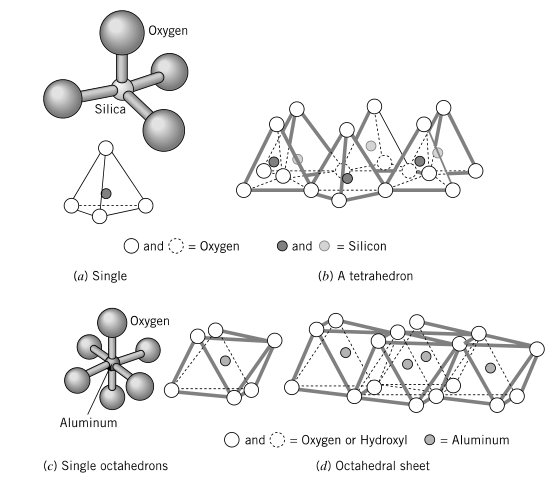
\includegraphics[scale=0.37]{Argile_1}
\caption{Feuillets}
\label{fig:argile1}
\end{subfigure}
\begin{subfigure}[h]{0.45\textwidth}
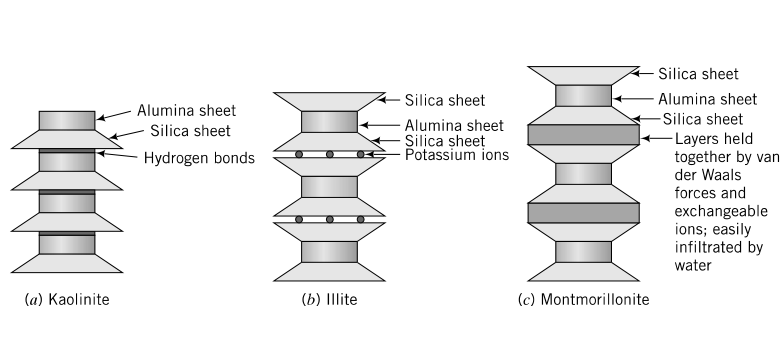
\includegraphics[scale=0.32]{Argile_2}
\caption{Types}
\label{fig:argile2}
\end{subfigure}
\caption{Structure de l'argile}
\end{figure}

L'argile possède une interaction particulière avec l'eau. Les faces des feuillets sont négativement chargée et tendent à attirer les cations présents dans l'eau ainsi que les dipôles d'eau. Cela forme une \textit{double couche} de dipôles qui attirent à leur tour d'autres dipôles et ainsi de suite (figure~\ref{fig:couche}). Le phénomène s'estompt assez vite avec la distance. Cette eau attirée à la surface de l'argile est dite adsordée. Ce comportement est responsable des propriétés de l'argile, notamment sa plasticité, son comportement face à la compression et au cisaillement.

\begin{figure}[ht]
\centering
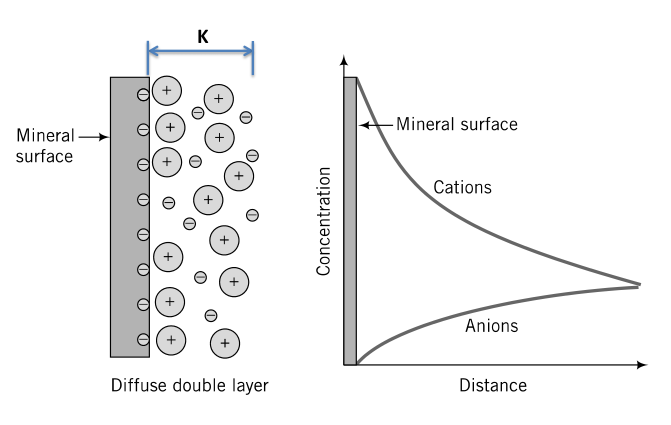
\includegraphics[scale=0.35]{Double_couche.png}
\caption{Eau adsordée}
\label{fig:couche}

\end{figure}

Les sols cohérents tels que l'argile peuvent avoir une structure bord à bord, dite \textit{floculée} (figure~\ref{fig:struc}a), ou face à face, dite \textit{dispersée} (figure~\ref{fig:struc}b).

\begin{figure}[ht]
\centering
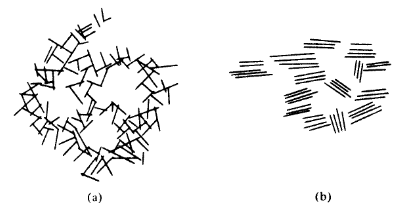
\includegraphics[scale=0.5]{Structure_argile.png}
\caption{Structures des sols cohérents}
\label{fig:struc}
\end{figure}

\section{Caractéristiques des sols}
\subsection{Taille des particules}
Le sol est composé de particules de différentes tailles (figure~\ref{fig:size1}).
\begin{figure}[h]
\centering
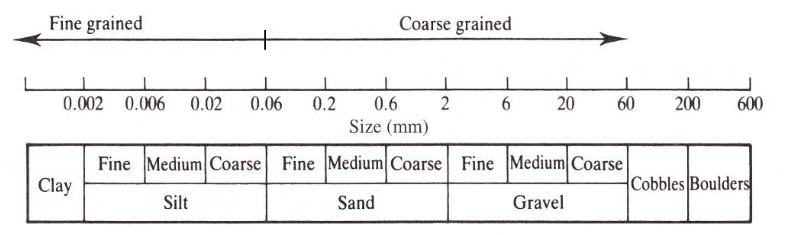
\includegraphics[scale=0.4]{size_1.png}
\caption{Tailles des éléments du sol}
\label{fig:size1}
\end{figure}
Pour pouvoir caractériser un sol, il est nécessaire de séparer les éléments en fonction de leur tailles. Pour les éléments plus grand que \unit{0.06}{\milli\meter}, cela peut se faire à l'aide de tamis dont les mailles sont de plus en plus petites. La masse de particules récupérées dans chaque tamis est pesée. Pour les particules plus petites, il faut recourir à la sédimentométrie. Cette technique consiste à mettre les grains restant en solution. Ceux-ci précipitent plus ou moins vite en fonction de leur taille et de leur poids spécifique.
Une fois ces tests réalisé, on peut réaliser un diagramme de distrubution (figure~\ref{fig:size2}. Celui-ci exprime le pourcentage (en masse) de grains plus petits qu'un certain diamètre. On peut donc en définir $D_{60}$ et $D_{10}$ qui correspondent au pourcentage de particules dont le diamètre est plus petit que 60 et \unit{10}{\milli\meter} respectivement. On appelle coefficient d'uniformité $UC$ le rapport entre ces deux diamètres : $UC = \frac{D_{60}}{D_{10}}$. Il est compris entre 1 et l'infini et diminue plus l'uniformité augmente.

\begin{figure}[ht]
\centering
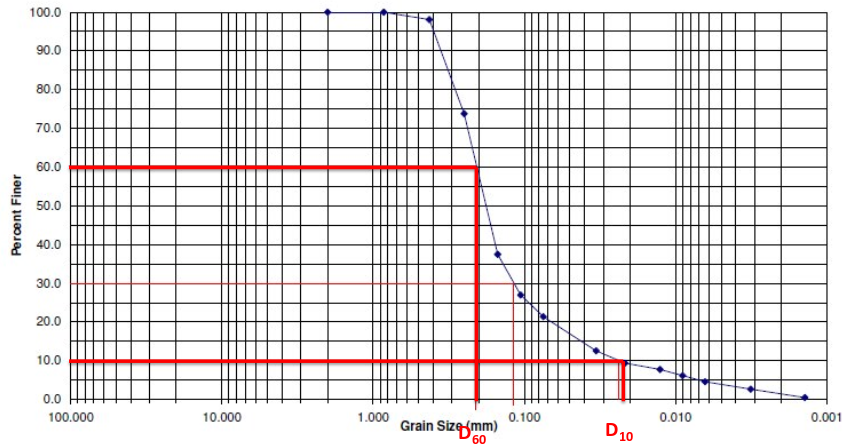
\includegraphics[scale=0.40]{size_2.png}
\caption{Diagramme de répartition ds tailles}
\label{fig:size2}
\end{figure}



\subsection{Relations masse-volume}
Le sol est constitué de grains entre lesquels se trouvent des vides. Ces vides peuvent être comblés soit par de l'eau, soit par de l'air. C'est pourquoi, dans le sol, trois états cohabitent : solide, liquide et gaz (figure~\ref{fig:volumesol}).
\begin{figure}[ht]
\centering
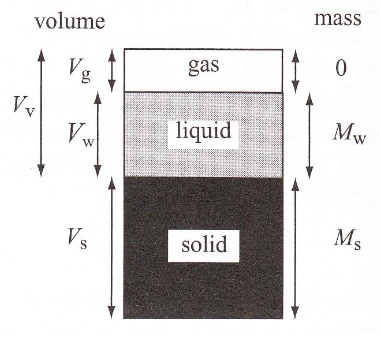
\includegraphics[scale=0.40]{volume_sol.png}
\caption{Constitution élémentaire d'un sol}
\label{fig:volumesol}
\end{figure}

Le volume total du sol $V$ est donné par : $$V = V_s + V_v = V_s + V_w + V_g$$
où $V_s$ est le volume de solide, $V_v$ le volume occupé par les vides et $V_w$ et $V_g$ les volumes occupés respectivement par l'eau et le gaz.
Le poids total $W$ est donné par : $$W = W_s + W_w$$
où $W = M*g$, $W_s$ et $W_w$ sont les poids du sol et de l'eau.
On notera que le poids de l'air est négligé.
Les poids volumique sont habituellement exprimé en \unit{\kilo\newton\per\cubic\meter} et le poids volumique de l'eau $\gamma_w$ vaut \unit{9.81}{\kilo\newton\per\cubic\meter}.

\paragraph*{Poids volumique $\gamma$} Correspond au rapport entre le poids et le volume d'un, les trois phases confondues : $$\gamma = \frac{W}{V} = \frac{W_s + W_w}{V_s + V_w + V_g}$$
Le poids volumique s'obtient en pesant un échantillon dont le volume est connu.
\paragraph*{Poids spécifique $\gamma_s$} Est le rapport entre le poids des particules solides et le volume occupé par celles-ci, vides non compris : $$\gamma_s = \frac{W_s}{V_s}$$
La plupart des sables ont un poids spécifique d'environ \unit{26}{\kilo\newton\per\cubic\meter} et de \unit{27}{\kilo\newton\per\cubic\meter} pour une argile.
La détermination du poids spécifique en laboratoire se fait à l'aide d'un pycnomètre. Le sol est d'abord pesé sec et ensuite pesé un fois saturé. Il est donc possible de déduire le volume occupé par le solide.
\paragraph*{Poids volumique sec $\gamma_d$} Peut être défini comme le poids des solides par unité de volume : $$\gamma_d = \frac{W_s}{V} = \frac{W_s}{V_s + V_w + V_g}$$
Celui des sables est généralement de \unit{16}{\kilo\newton\per\cubic\meter}.
\paragraph*{Poids spécifique saturé $\gamma_{sat}$} Lorsque le sol est saturé, tous les vides sont occupés par de l'eau, donc $V_v = V_w$ : $$\gamma_{sat} = \frac{W_{sat}}{V} = \frac{W_s + W_w}{V_s + V_w}$$
Celui des sables est généralement de \unit{20}{\kilo\newton\per\cubic\meter}.
\paragraph*{Poids volumique déjaugé $\gamma'$} Utilisé lorsqu'un sol est submergé : $$\gamma' = \gamma_{sat} - \gamma_w$$
\paragraph*{Teneur en eau $w$} Est le rapport entre le poids d'eau et de solide, s'exprime en \% : $$w = \frac{W_w}{W_s}$$
La détermination de la teneur en eau en laboratoire se fait en pesant un sol avant et après l'avoir séché entre 100 et \unit{105}{\celsius}. La différence des deux poids donne le poids de l'eau et le poids après séchage le poids des solides. 
\paragraph*{Indice des vides $e$} Est le rapport entre le volume des vides et le volume des solides et n'a pas d'unités : $$e = \frac{V_v}{V_s} = \frac{V_w + V_g}{V_s}$$
\paragraph*{Porosité $n$} Est le rapport entre le volume des vides et le volume total et est exprimée en \%. Ne peut pas dépasser 100\% : $$n = \frac{V_v}{V} = \frac{V_w + V_g}{V_s + V_w + V_g}$$
Porosité et indices des vides sont liés par la relation : $$n = \frac{e}{1+e}$$
\paragraph*{Degré de saturation $S_r$} Est le rapport entre le volume d'eau et de vides. S'exprime en \%, un sol est sec à 0\% et saturé à 100\% : $$S_r = \frac{V_w}{V_v} = \frac{V_w}{V_w + V_g}$$
\paragraph*{Densité relative $D_{r,e}$ ou $D_{r,n}$} Exprime la relation entre l'état le plus compact et le moins compact d'un sol : $$D_{r,e} = \frac{e_{max} - e}{e_{max} - e_{min}}$$ et $$D_{r,n} = \frac{n_{max} - n}{n_{max} - n_{min}}$$

\subsection{Consistance}
La consistance d'un sol dépend de son contenu en eau (figure~\ref{fig:consistance}). Le sol peut se présenter sous plusieurs états : liquide, tel une boue; plastique, malléable et se laisse pétrir, se déforme sans fissures; semi-solide, avec retrait, se déforme avec fissures; solide, sans retrait, dur.
\begin{figure}[ht]
\centering
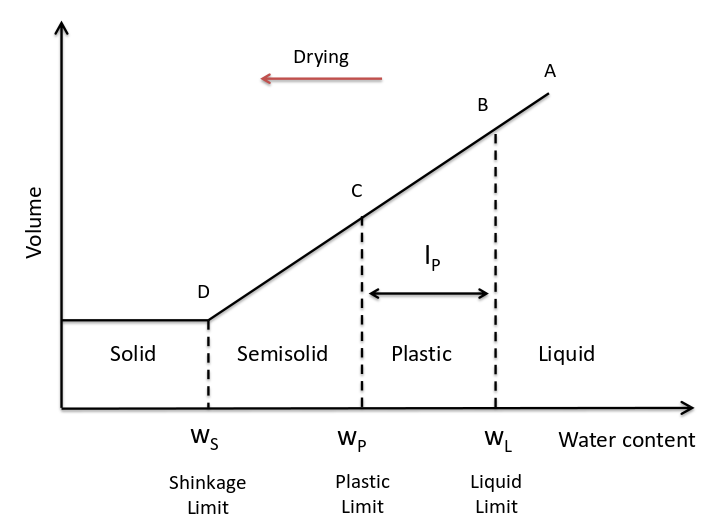
\includegraphics[scale=0.35]{consistance.png}
\caption{Consistance}
\label{fig:consistance}
\end{figure}
On peut donc définir différentes limites entre ces états : la limite de retrait $w_s$, la limite de plasticité $w_p$ et la limité de liquidité $w_l$.
La limited de liquidité est déterminée à l'aide de la méthode de la coupelle de Casagrande. Un échantillon de sol est placé dans la coupelle dans lequel une rainure est faite. La coupelle est ensuite soulevée puis laissée retomber avec une came. L'opération est répétée jusqu'à ce que la rainure se ferme. La limite de liquidité est définie comme la teneur en eau pour laquelle la fermeture se fait en 25 coups.

La limite de placticité peut être obtenue de différentes manières. Premièrement elle est déterminée comme la teneur en eau la plus basse pour laquelle il est possible de rouler le sol en rouleaux de \unit{3}{\milli\meter} sans les casser. Cette technique peut paraitre imprécise mais est très répétitive et satisfaisante. Une deuxème méthode consiste à faire tomber un cône sur la pointe dans un échantillon de sol. Le cône s'enfonce plus ou moins en fonction de la teneur en eau et d'une certaine hauteur lorsque le sol est à la limite de plasticité.


\paragraph*{Indice de plasticité} Par définition, la teneur en eau qui sépare l'était liquide de l'état plastique : $$I_p = w_l - w_p$$
\paragraph*{Indice de liquidité} Permet de caractérisé l'échantillon par rapport aux limites du domaine de plasticité : $$I_l = \frac{w - w_p}{w_l - w_p}$$

\subsection{Teneur en matières organiques et carbonatées}
Le sol contient souvent de la matière organique (humus,...) ou calcareuse. 
\paragraph*{Teneur en matière organique (\textit{Organic Content}) $OC$} Déterminée en observant la différence de masse entre un échantillon seché avant et après réaction avec de l'\ce{H2O2}.
\paragraph*{Teneur en matière carbonatées (\textit{Carbonates Content}) $CC$} Déterminée en observant la différence de masse entre un échantillon seché avant et après réaction avec du \ce{HCl}.

\section{Classification du sol}
Le sol peut être classé de différentes manières. En fonction de la proportion de particules d'un certain diamètre, de la teneur en matières organiques/carbonatées, de l'indice de plasticité,...


\chapter{Interaction sol-eau}
\section{L'eau dans le sol}
\label{chap:eau}

Hormis l'eau de constitution du sol, l'eau peut être présente sous différentes formes. 
\begin{itemize}
\item L'eau phréatique : présente continue d'eau souterraine, remplissant les vides et fissures du sol.
\item L'eau capillaire : la capillarité est la capacité d'un liquide de se déplacer en opposition aux forces externes (gravité) grâce aux forces intermoléculaires entre le liquide et les surfaces du solide. 
\end{itemize}

Les sols sont aussi classés selon leur perméabilité : 
\begin{itemize}
\item Aquifère : entité perméable comportant une zone saturée et contenant assez d'eau pour être exploitée. Perméabilité : \unit{\power{10}{-5}}{\meter\per\second}.
\item Aquitard : entité peu perméable, mais conductrice d'eau en faible quantité, exploitation très limitée. Perméabilité : de \power{10}{-5} à \unit{\power{10}{-7}}{\meter\per\second}.
\item Aquiclude : entité imperméable, très peu conductrice d'eau. Perméabilité : plus petite que \unit{\power{10}{-7}}{\meter\per\second}.
\end{itemize}

La pression interstitielle $u$ est définie comme le poids la hauteur d'eau au dessus du point : $$u = \gamma_w h_w$$
Le niveau piézométrique est le niveau auquel l'eau s'établirait si on introduisait un tube dans la poche d'eau.

\section{Ecoulement de l'eau}
Selon la loi de Bernouilli, le potentiel de l'eau est donné par : $$P = z + \frac{u}{\gamma} + \frac{v^2}{2g}$$ où $z$ est la hauteur par rapport à une référence, $u$ la pression interstitielle et $v$ la vitesse d'écoulement.

Dans le cas d'écoulement d'eau dans le sol, la vitesse d'écoulement est faible et peut être négligée, ce qui donne : $$P = z + \frac{u}{\gamma} = z + h$$ où $h$ est la hauteur piézométrique (figure~\ref{fig:bernouilli}

\begin{figure}[ht!]
\centering
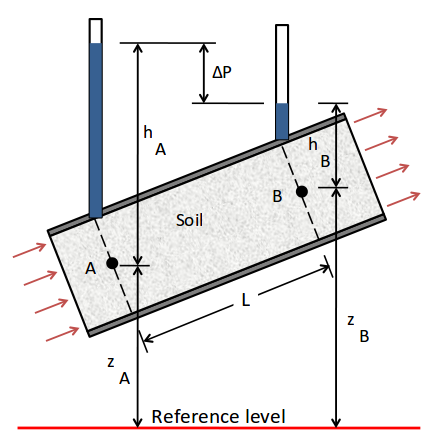
\includegraphics[scale=0.35]{bernouilli.png}
\caption{Illustration du flux d'eau dans un sol}
\label{fig:bernouilli}
\end{figure}

Entre les points A et B, il y a une différence de potentiel $\Delta P = z_A - z_B + h_A - h_B$. Un flux se produit seulement si il y a une différence de potentiel. Le flux se déplace du point au potentiel le plus haut jusqu'au point au potentiel le plus bas.

Nous pouvons définir le gradient hydraulique $i$ qui est, par définition le rapport entre la différence de potentiel et la distance parcourue : $$i = \frac{\Delta P}{L}$$
De plus, le débit est donné par : $$q = \frac{\Delta V}{\Delta t} = v A$$ où $\Delta V$ est le volume de l'échantillon traversé, $A$ sa section et $v$ la vitesse de percolation. 
\bigbreak
A partir de là, il est possible d'établir la loi de Darcy : $$v = k i$$ où k est le coefficient de perméabilté (coefficient de conductivité hydraulique) dont les unités sont des \unit{\meter\per\second}.

\subsection{Détermination de de $k$}
\label{chap:k}
\begin{figure}[ht!]
\begin{subfigure}[h!]{0.45\textwidth}
\centering
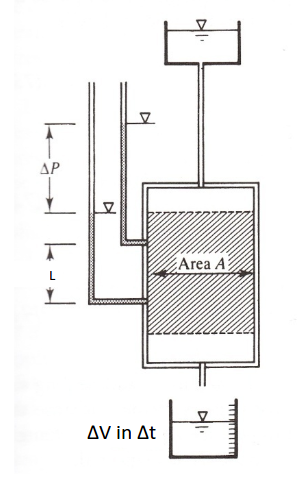
\includegraphics[scale=0.40]{permeametre_constant.png}
\caption{Niveau constant}
\label{fig:constant}
\end{subfigure}
\begin{subfigure}[h!]{0.45\textwidth}
\centering
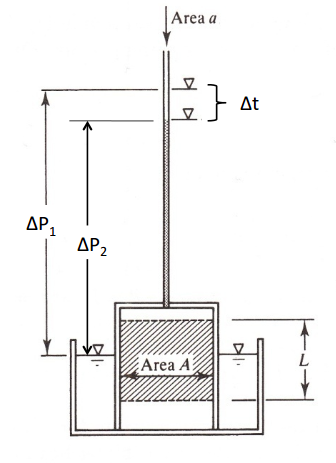
\includegraphics[scale=0.40]{permeametre_variable.png}
\caption{Niveau variable}
\label{fig:variable}
\end{subfigure}
\caption{Détermination de $k$}
\end{figure}

\paragraph*{Perméamètre à niveau constant} L'alimentation se fait d'un réservoir placé en hauteur (figure~\ref{fig:constant}). Lorsqu'un écooulement s'établit, on récolte un volume $\Delta V$ dans le récipient du bas en un temps $\Delta t$. Par la loi de Darcy le débit vaut : $$\frac{\Delta V}{\Delta t} = q = v A = k i A = k \frac{\Delta P}{L} A$$ Le coefficient de perméabilité est donc donné par : $$k = \frac{\Delta V L}{\Delta t A \Delta P}$$
Cet essai est approprié pour des sols à perméabilité élevée ($k$ > \unit{\power{10}{-5}}{\meter\per\second}) et l'échantillon doit être saturé avant l'essai.

\paragraph*{Perméamètre à niveau variable} Cet essai est utilisé plutôt pour des sables très fins, des argiles et des limons. En effet, il ne serait pas possible de faire passer un volume d'eau à travers un échantillon dans un temps convenable, une partie de l'eau aurait le temps de s'évaporer. Ici, le réservoir suppérieur est remplacé par un tube capillaire et lorsque l'eau s'écoule dans l'échantillon, le niveau du tube diminue (figure~\ref{fig:variable}). Sur un intervalle de temps $dt$, le niveau diminue de $dP$, le volume écoulé s'écrit donc $-a dP$. le débit à travers l'échantillon vaut : $$A k \frac{\Delta P}{L} = A v = q = -a \frac{dP}{dt}$$
En intégrant entre deux instants de prises de mesures : $$A \frac{k}{L} \int^{t_2}_{t_1} dt = -a \int^{\Delta P_2}_{\Delta P_1} \frac{dP}{\Delta P} $$ 
Ce qui donne : $$k = \frac{a L}{A \Delta t} \ln\frac{\Delta P_1}{\Delta P_2}$$
Ce coefficient est aussi appelé coefficient de perméabilité intrinsèque.

\paragraph*{Formule empirique de Hazen} $$k : 116(0.7 + 0.03 T)d_{10}^2$$ où $d_{10}^2$ est le diamètre actif des grains, correspondant à un passant de 10\% dans la courbe granulométrique.

\paragraph*{Autres formules utiles} Le coefficient à une température $T$ est donné par : $$k_{20} = k_T \frac{\eta_T}{\eta_{20}}$$ où $\eta_T$ est la viscosité dynamique de l'eau à la température $T$.

Le coefficient de perméabilité physique est défini par : $$k_0 = k \frac{\eta}{\gamma_w}$$

\subsection{Ecoulement à travers plusieurs sols différents}

\begin{figure}[ht!]

\begin{subfigure}[h!]{0.45\textwidth}
\centering
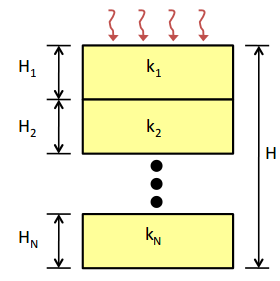
\includegraphics[scale=0.40]{vertical.png}
\caption{Flux vertical}
\label{fig:vertical}
\end{subfigure}
\begin{subfigure}[h!]{0.45\textwidth}
\centering
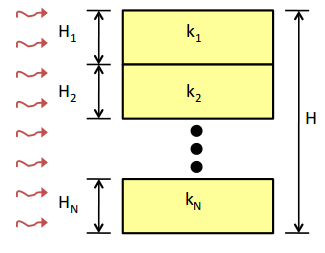
\includegraphics[scale=0.42]{horizontal.png}
\caption{Flux horizontal}
\label{fig:horizontal}
\end{subfigure}
\caption{Flux à travers différentes couches}
\end{figure}

\paragraph*{Flux vertical} Comme représenté à la figure~\ref{fig:vertical} le flux passe successivement dans différents couches de sols différents. La vitesse d'écoulement est donc la même à travers chaque couche : $$v = v_{éq} = k_{éq} i_{éq} = k_{éq} \frac{\Delta P_{éq}}{H} = v_i = k_i i_i = k_i \frac{\Delta P_i}{H}$$
De plus : $$\Delta P_{éq} = \sum \Delta P_i$$
Nous avons donc : $$\frac{H v}{k_{éq}} = \sum\frac{H_i v}{k_i}$$
Finalement : $$k_{éq} = \frac{H}{\sum\frac{H_i}{k_i}}$$

\paragraph*{Flux horizontal} Comme représenté à la figure~\ref{fig:horizontal}, le flux est parallèle aux différentes couches et chaque couche à le même gradient hydraulique $i$. Le débit est donné par : $$q = H L v_{éq} = H L k_{éq} i$$ où $L$ est l'épaisseur de la couche, $H L$ est donc la section de l'échantillon.
Ce débit est la somme de chaque débit $q_i$ : $$q = \sum H_i L k_i i$$
Ce qui donne : $$k_{éq} H = \sum k_i H_i$$
Enfin : $$k_{éq} = \frac{\sum k_i H_i}{H}$$

\section{Ecoulement d'eau en 2D}
Comme représenté à la figure~\ref{fig:ec2d}, le volume d'eau entrant dans l'élément infinitésimal est donné par : $$v_x dy dz + v_y dx dz$$ tandis que le volume sortant est donné par : $$\left( v_x + \frac{\delta v_x}{\delta x}dx \right) dy dz + \left( v_y + \frac{\delta v_y}{\delta y}dy \right) dx dz$$ 

\begin{figure}[ht!]
\centering
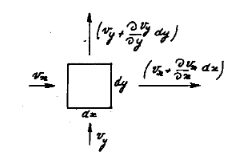
\includegraphics[scale=0.75]{ecoulement_2d.png}
\caption{Ecoulement dans un élément infinitésimal}
\label{fig:ec2d}
\end{figure}

Si le volume de l'élément reste constant, le flux d'entrée est égal au flux de sortie : $$\frac{\delta v_x}{\delta x}dx dy dz + \frac{\delta v_y}{\delta y}dy dx dz = 0$$

De la loi de Darcy, nous savons : $$v_x = k_x i_x = k_x \frac{\delta P}{\delta x}$$ 

L'équation devient donc : $$k_x \frac{\delta^2 P}{\delta x^2} = k_y \frac{\delta^2 P}{\delta y^2}$$ qui correspond à l'équation de Laplace. 

Pour un sol isotrope ($k_x = k_y$), l'équation devient : $$\frac{\delta^2 P}{\delta x^2} = \frac{\delta^2 P}{\delta y^2}$$

\subsection{Calcul du débit}
L'étude de l'écoulement se fait en utilisant un réseau (figure~\ref{fig:ec2d2}) de deux courbes : des équipotentielles (le potentiel est le même le long de la ligne) et des lignes de courant (chemin que tend l'autre à prendre). Le débit est constant dans un tube de courant (entre deux lignes de courant), et, dans notre cas, le réseau est carré. Si $N_f$ est le nombre de tubes de courant, le débit est donné par : $$q = N_f \delta q = N_f k i \delta b$$ 
\begin{figure}[ht!]
\centering
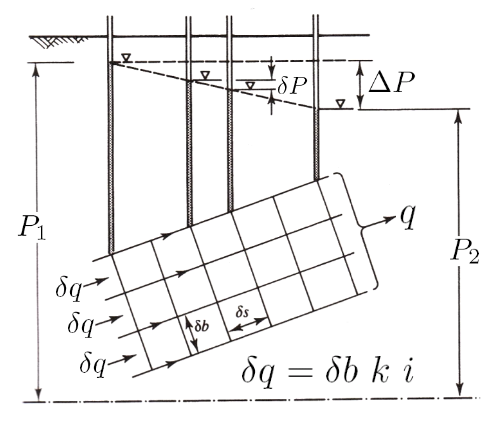
\includegraphics[scale=0.40]{groundwaterflow.png}
\caption{Ecoulement en 2D}
\label{fig:ec2d2}
\end{figure}
De plus, le réseau étant carré, la chute de potentiel $\delta P$ est conctante d'équipotentielle en équipotentielle. Si $N_d$ est le nombre de chutes de potentiel (entre deux équipotentielles) : $$\delta P = \frac{\Delta P}{N_d}$$

Le gradient hydraulique entre deux équipotentielles est donc donné par : $$i = \frac{\delta P}{\delta s} = \frac{\Delta P}{N_d \delta s}$$

Nous pouvons maintenant définir le flux dans le réseau comme : $$q = k \frac{N_f}{N_d}\Delta P$$

\subsection{Flux dans un milieu anisotrope}
Dans ce cas, l'équation de Laplace : $$k_x \frac{\delta^2 P}{\delta x^2} = k_y \frac{\delta^2 P}{\delta y^2}$$ peut être réécrite comme : $$\frac{\delta^2 P}{\frac{k_y}{k_x}\delta x^2} \frac{\delta^2 P}{\delta y^2} = 0$$

En définissant $x' = x\sqrt{\frac{k_y}{k_x}}$, l'équation devient : $$\frac{\delta^2 P}{\delta x'^2} + \frac{\delta^2 P}{\delta y^2} = 0$$

Pour résoudre ce genre de problème et pouvoir en faire une résolution graphique avec une réseau, il faut appliquer une distorsion de l'axe des $y$ : $$y' = y\sqrt{\frac{k_x}{k_y}}$$

Le flux est alors donné par : $$q = \sqrt{k_x k_y}\frac{N_f}{N_d}\Delta P$$


\chapter{Contraintes}

Ce chapitre couvre uniquement le cas des contraintes verticales, normales. Celles-ci sont définies comme le poids de colonne de sol au dessus d'un point (figure~\ref{fig:contvert}), et en se rappelant que $W = \gamma V$ : $$\sigma_v = \frac{W}{A} = \frac{\gamma V}{A} = \gamma h$$ 

Les unités sont des \unit{\kilo\newton\per\meter\squared} = \unit{\kilo\pascal}.

\begin{figure}[ht!]
\centering
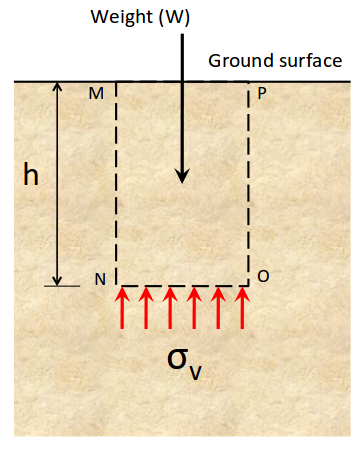
\includegraphics[scale=0.40]{contrainte_verticale.png}
\caption{Contrainte verticale}
\label{fig:contvert}
\end{figure}

\section{Sol sec} 
Lors du calcul des contraintes dans un sol sec (figure~\ref{fig:solsec}), il faut prendre le poids volumique sec $\gamma_d$. La contrainte à une profondeur $z$ est simplement donnée par : $$\sigma_v = \gamma_d z$$

\begin{figure}[ht!]
\centering
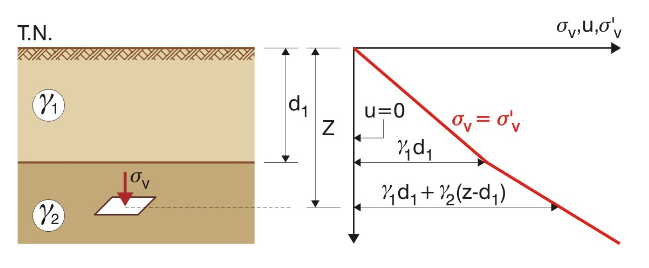
\includegraphics[scale=0.45]{contr_sec.png}
\caption{Sol sec}
\label{fig:solsec}
\end{figure}

Si il y a plusieurs couches de sols différents, il faut prendre en compte les contraintes de chaque couche. La contrainte à une profondeur $z_n$ depuis le sol en se trouvant dans la couche $n$ est donnée par : 
$$\sigma_v(z_n) = \sum\limits_{i=1}^{n-1} \left( \gamma_{d_i} h_i + \left( z - \sum\limits_{i=1}^{n-1} h_i \right)\gamma_{d_n} \right)$$

\section{Présence d'eau}
Dans ce cas, la pression interstitielle $u$ est non nulle et se calcule de la même façon que précédemment : $u = \gamma_w h_w$. Il est important de la prendre en compte, la contrainte totale est maintenant la contrainte des particule plus la contrainte de l'eau. La contrainte apparente subie par le sol est définie par : $$\sigma'_v = \sigma_v - u$$

Différents cas de figures peuvent se présenter.

\subsection{Sol submergé}
Si le sol est situé sous une couche d'eau d'une hauteur H (figure~\ref{fig:solsub}), le sol en dessous est saturé, il faut donc prendre en compte le poids volumique saturé du sol $\gamma_{sat}$. 

\begin{figure}[ht!]
\centering
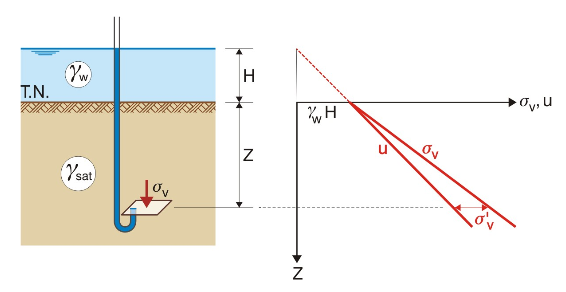
\includegraphics[scale=0.45]{contr_sub.png}
\caption{Sol submergé}
\label{fig:solsub}
\end{figure}

La contrainte à une profondeur $z$ est donnée par : $$\sigma_v = \gamma_w H + \gamma_{sat}z$$
et la pression interstitielle est donnée par : $$\gamma_w (H+z)$$

La contrainte apparente et la différence des deux et vaut : $$\sigma_v' = (\gamma_{sat}-\gamma{w})z = \gamma'z$$ où $\gamma' = \gamma_{sat}-\gamma{w}$ est le poids volumique déjaugé.

Dans ce cas-ci, il faut bien faire attention à à prendre en compte le poids de l'eau au dessus du sol lors du calcul de la contrainte. Cependant, le poids de l'eau n'augmente pas, même si l'on descend en profondeur, la contrainte associée à l'eau restera constante ($\gamma_w H$). Néanmoins la pression interstitielle continue d'augmenter avec la profondeur vu que le sol est saturé.


\subsection{Sol sec au dessus d'une couche saturée (pas d'ascencion capillaire)}
Une couche de sol sec d'épaisseur $D$ est située aus dessus d'une couche saturée (figure~\ref{fig:soltop}. Il faut donc utilsé $\gamma_d$ pour la première couche et $\gamma_{sat}$ pour la seconde. 

\begin{figure}[ht!]
\centering
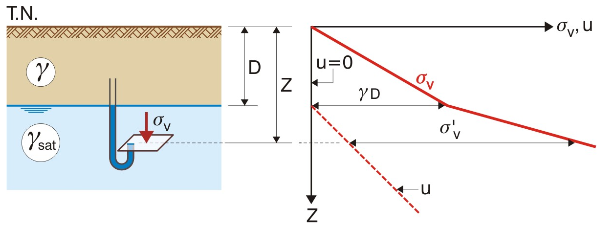
\includegraphics[scale=0.45]{contr_top.png}
\caption{Couche sèche au dessus d'une couche saturée}
\label{fig:soltop}
\end{figure}

Dans la première couche ($z<D$), il n'y a pas d'eau, donc pas de pression interstitielle, la contrainte est donc donnée par : $$\sigma_v = \sigma_v' = \gamma_d z$$

Dans la seconde couche ($z>D$), la contrainte est la somme de la contrainte due au sol sec (constante !) et de celle liée au sol saturé : $$\sigma_v = \gamma_d H + \gamma_{sat}(z-D)$$

La pression interstielle n'es plus nulle et vaut : $$\gamma_w (z-D)$$

La contrainte apparente est donnée par : $$\sigma_v' = \gamma_d D + \gamma'(z-D)$$


\subsection{Sol saturé - nappe libre au repos avec ascension capillaire}

Dans ce cas, une nappe est située en dessous d'une couche de sol homogène (figure~\ref{fig:solcap}). Le niveau phréatique s'établit à une profondeur $D$. Sous ce niveau, le sol est saturé. Au dessus, il y a ascension capillaire et on suppose que la hauteur de l'ascension est supérieure à $D$, le sol est donc aussi saturé. 

\begin{figure}[ht!]
\centering
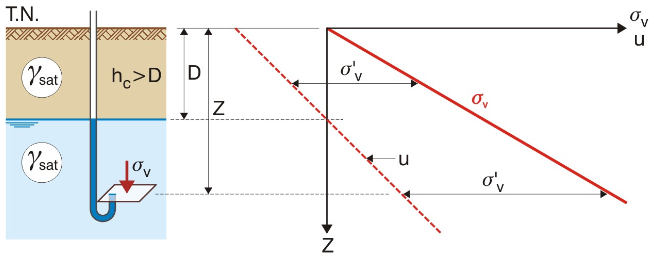
\includegraphics[scale=0.37]{contr_cap.png}
\caption{Nappe libre}
\label{fig:solcap}
\end{figure}

Etant donné que les deux couches du (même) sol sont saturées, il faut prendre en compte $\gamma_{sat}$ pour les deux. La contrainte est donc linéaire à travers les deux couches et vaut à une profondeur $z$ : $$\sigma_v = \gamma_{sat} z$$

La pression interstitielle s'annule au niveau phréatique ($z = D$) et varie linéairement avec la profondeur : $$u = \gamma_w (z-D)$$

On observe que $u$ sera négatif au dessus du niveau phréatique, l'eau est mise en dépression, ce qui illustre bien l'ascension capillaire.

La contrainte apparente est : $$\sigma_v' = \gamma'z + \gamma_w D$$

\subsection{Nappe sous un sol imperméable - soufflage}

Lorsqu'une nappe est située sous un sol imperméable, il est possible que le niveau phréatique soit au dessus du niveau de la nappe (figure~\ref{fig:solsou}). Il y a une couche d'argile de profondeur $D$ sous laquelle se trouve un sol saturé par une nappe dont le niveau s'établit à une distance $d$ de la surface.

\begin{figure}[ht!]
\centering
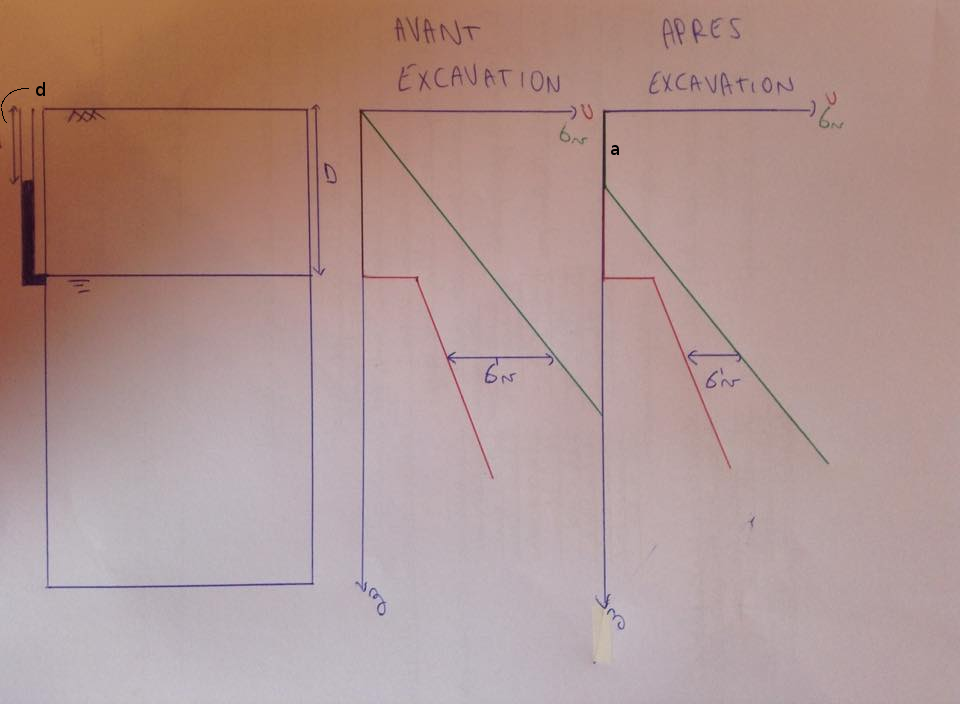
\includegraphics[scale=0.40]{contr_sou.png}
\caption{Nappe sous couche imperméable}
\label{fig:solsou}
\end{figure}

Dans la couche d'argile imperméable, la pression interstitielle est nulle et les contraintes sont données par : $$\sigma_v = \sigma_v' = \gamma_{d_1} z$$

Juste en dessous de la deuxième couche, la pression interstitielle augmente d'un coup d'une valeur : $(D-d)\gamma_w$. A une profondeur $z$, elle vaut : $$u = (D-d)\gamma_w + (z-D)\gamma_w = (z-d)\gamma_w$$

La contrainte vaut, quant à elle : $$\sigma_v = D\gamma_{d_1} + (z-D)\gamma_{sat_2}$$ 

La contrainte effective, diminue brusquement au niveau de D puis son expression est : $$\sigma_v' = D\gamma_{d_1} + (z-D)\gamma_{sat_2} - (z-d)\gamma_w = D(\gamma_{d_1} - \gamma_{sat_2}) + d \gamma_w  + z(\gamma_{sat_2}-\gamma_w)$$

Par définition, le soufflage survient lorsque $\sigma_v' = 0$ ce qui revient à dire lorsque $\sigma_v = u$, en une certaine profondeur. Dans ce cas, les forces du à la pression interstitielle de la nappe confinée seront plus grande que la contrainte du sol au dessus, les contraintes entre les grains deviennent nulles. Il y aura une instabilité du sol (sables mouvants). il est intéressant de savoir prévoir ce phénomène dans le cas d'excavations. En effet, plus on creuse, plus on diminue la contrainte de la couche supérieure imperméable. Comme on peut le voir sur le graphe de droite de la figure~\ref{fig:solsou}, si on creuse d'une profondeur $a$, la contrainte est nulle jusqu'à cette profondeur. Le point critique est à une profonceur $D$, c'est là que $\sigma_v'$ atteint un minimum.

Il est possible de trouver la profondeur maximale $a'$ d'excavation en égalant $\sigma_v$ et $u$ à la profondeur $z = D$ : $$\sigma_v = (D-a')\gamma_{d_1} + (z-D)\gamma_{sat_2} = (D-a')\gamma_{d_1}$$
et $$u = (D-d)\gamma_w + (z-D)\gamma_w = (D-d)\gamma_w$$
La profondeur maximale est donc donnée par : $$a' = D - \frac{(D-d)\gamma_w}{\gamma_{d_1}}$$

\section{Ajout d'une charge}
Si l'on ajoute une charge sur un sol, celui-ci peut réagir de deux manières. 

\begin{figure}[ht!]
\centering
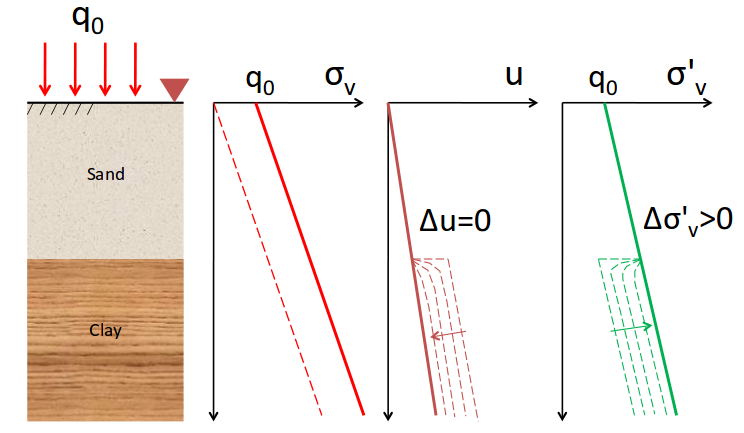
\includegraphics[scale=0.30]{load.png}
\caption{Ajout d'une charge sur un sol}
\label{fig:load}
\end{figure}

Comme le sable qui, lui, peut éjecter/capter facilement de l'eau de ses pores, l'eau peut drainer à travers le sol la pression interstitielle ne changera aps après application de la charge (figure~\ref{fig:load}). L'argile, quand à lui, dans un premier temps, ne peut pas éjecter d'eau de ses pores, la pression interstitielle va donc augmenter. La contrainte effective, elle ne change pas. Avec le temps, l'argile va petit à petit éjecter l'eau de ses pores et rejoindre le même état que le sable. A court terme, l'eau ne peut pas drainer à travers l'argile mais, à long terme, celle-ci en est capable.



\chapter{Compression}
\label{chap:compr}

Dans ce chapitre, nous traiterons uniquement des contraites normales;
Le sol est une matériau de solides et de vides. Si une contrainte est appliquée sur un échantillon, les molécules vont se réarranger, l'espace occupé par les vides va se réduire, expulsant une certaine quantité de vides (air et eau si le sol en contient). Le volume total diminue ainsi que la masse si de l'eau est expulsée. De ce fait, l'indice des vides $e = \frac{V_v}{V_s}$ diminue également. On observe que l'indice des vides est inversément proportionnel à la contrainte.

L'étude de la compressibilité se fait à l'aide d'un test \oe{}dométrique. L'échantillon est placé dans un anneau rigide entre deux pierres poreuses (qui laissent passer l'eau). Une contrainte est appliquée par paliers successifs sur le eau de l'échantillon. L'abaissement de hauteur est mesuré après la stabilisation et les résultats sont portés sur un diagramme indice des vides-contrainte (figure~\ref{fig:comprplot})

\begin{figure}[ht!]
\centering
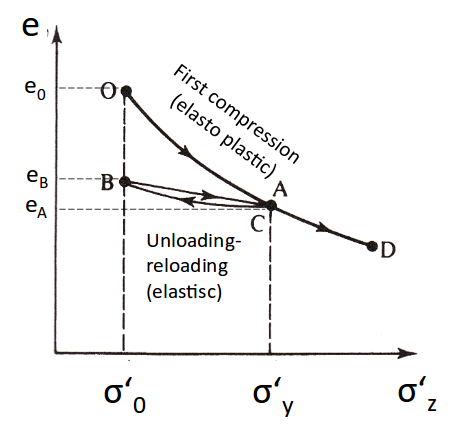
\includegraphics[scale=0.35]{compr_plot.png}
\caption{Graphe de $e$ en fonction de $\sigma'$}
\label{fig:comprplot}
\end{figure}

Lorsqu'on applique pour la première fois une charge sur un sol, la déformation est élastoplatique et suis la courbe $OA$. Arrivé au point $A$, si l'on retire la charge, une partie de la déformation reste, l'échantillon ne revient pas à son volume initial. Sur cette partie de la courbe $BA$, la déformation est élastique, tant qu'on ne dépasse pas la contrainte en $A$, on restera sur cette courbe, et, si l'on enlève la charge, on se retrouvera au point $B$. Si l'on dépasse la charge au point A, on retrouve un comportement élastplastique et ainsi de suite. 
La partie élastoplastique de la courbe ($OD$) est appelée \textit{Normal Compression Line} (NCL) tandis que la partie élastique est appelée \textit{Unloading-Reloading Line} (URL).

\section{Préconsolidation}
Un sol est dit préconsolidé si, dans son passé, il a subi une contrainte $\sigma_y'$ supérieure à la contrainte $\sigma_0'$ qu'il connait actuellement. Cette contrainte de consolidation correspond à la contrainte marquant la transition entre une URL et NCl (point $A$). On appelle degré de préconsolidation le rapport de ces deux contraintes : $$Y_0 = \frac{\sigma_y'}{\sigma_0'}$$ Si il est supérieur à 1, le sol est préconsolidé, si il est égal à 1, le sol ne l'est pas. Si le sol n'est pas préconsolidé, lors de l'application d'une contrainte, le sol aura une déformation élastique et suivra la courbe $OD$ du diagramme. Si il est préconsolidé, il aura une déformation élastique et suivra la courbe $BA$ pour rejoindre la courbe $AD$ si la contrainte est suffisante.

\section{Tassement}
Si l'on se trouve sur une NCL, si le sol n'est pas préconsolidé, en échelle logarithmique, l'équation de la courbe peut être approximée par : $$e = e_0 - C_c \log(\sigma_z')$$
qui est une droite de pente $C_c$ (voir figure~\ref{fig:comprplot2}) où $C_c$ est l'indice de compressibilité.

\begin{figure}[ht!]
\centering
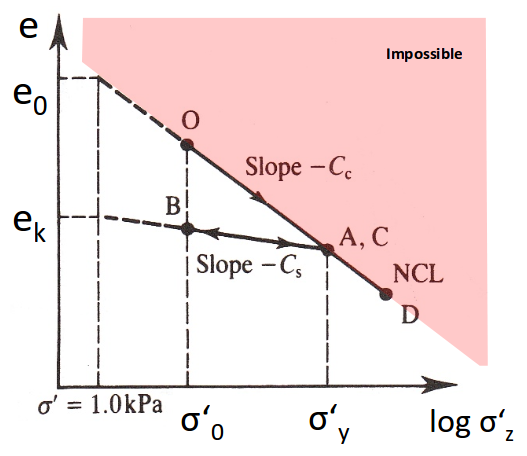
\includegraphics[scale=0.35]{compr_plot_2.png}
\caption{Allure simplifiée du graphe de $e$ en fonction de $\sigma'$ (échelle logarithmique)}
\label{fig:comprplot2}
\end{figure}

Il est possible de calculer le tassement du sol en reliant la variation de hauteur $s$ à la variation de volume $\Delta V$ : $$\frac{s}{H} = \frac{\Delta V}{V_0}$$ où $H$ et $V_0$ sont les hauteur et volume initiaux. Nous savons que $V_v = e V_s$, que $V = V_v + V_s$ et que $V_s$ est constant, donc :   
$$\frac{s}{H} = \frac{\Delta V}{V_0} = \frac{V_{0_v} + V_s + V_{f_v} + V_s}{V_{0_v} + V_s} = \frac{V_s(e_0 - e_f}{V_s(e_0 + 1)} = \frac{\Delta e}{1 + e_0}$$ 

En utilisant l'équation de la courbe, on obtient finalement : $$\frac{s}{H} = \frac{C_c}{1 + e_0}\log\frac{\sigma_f'}{\sigma_0'}$$ où  $\sigma_f'$ et $\sigma_0'$ sont les contraintes finale et initiale. 

Une formulation alternative est : $$ \frac{s}{H} = \frac{1}{C}\ln\frac{\sigma_f'}{\sigma_0'}$$ où $C$ est la constante de compressibilité. 

En faisant la correcpondance entre les deux formulation, nous avons : $$\frac{C_c}{1 + e_0}\log\frac{\sigma_f'}{\sigma_0'} = \frac{1}{C}\ln\frac{\sigma_f'}{\sigma_0'}$$	 

En exprimant les logarithmes dans la même base, nous avons : $$\frac{C_c}{1 + e_0}\log\frac{\sigma_f'}{\sigma_0'} = \frac{1}{C}\frac{\log\frac{\sigma_f'}{\sigma_0'}}{\log e}$$	 

De là, il est possible de trouver la correspondance entre $C_c$ et $C$ : $$C_c = \frac{1+e_0}{C\log e} \approx 2.3\frac{1+e_0}{C}$$

\section{Gonflement}

Si l'on se trouve sur une URL, le sol est préconsolidé, sa déformation est élastique et on se trouve sur la ligne $BA$ qui à comme équation, en échelle logarithmique : $$e = e_k - C_s \log(\sigma_z')$$ qui est une droite de pente $C_s$ (voir figure~\ref{fig:comprplot2}) où $C_s$ est l'indice de gonflement. 

Il est possible de calculer le gonflement suite au retrait de la contrainte en utilisant la formule : $$\frac{s}{H} = \frac{C_S}{1 + e_0}\log\frac{\sigma_f'}{\sigma_0'}$$ qui s'obtient de la même manière que pour le tassement.

Une formulation alternative est : $$ \frac{s}{H} = \frac{1}{A}\ln\frac{\sigma_f'}{\sigma_0'}$$ où $A$ est la constante de gonflement. De façon similaire à la relation liant $C_c$ et $C$, on obtient : $$C_s = \frac{1+e_0}{A\log e} \approx 2.3\frac{1+e_0}{A}$$

\paragraph*{Remarque} Si l'on se trouve sur une URL, et qu'on ajoute de la contrainte, on provoque un tassement, une compression, cependant, le tassement sera proportionnel à l'indice de gonflement (!) tant qu'on reste sur l'URL.

\section{Calcul du tassement}
Dans certains cas, il sera nécessaire de déterminer la contrainte de préconsolidation à partir de valeurs/graphe. Comme sur la figure~\ref{fig:comprreal}, une technique consiste à prendre l'intersection entre la courbe NCL et la bissectrice entre la tangente à l'URL et l'horizontale au point de la courbe avec le rayon minimum. Cependant, il n'est pas facile de trouver précisément le rayon minimum d'une courbe (surtout si celle-ci est tracée à partir d'un tableau de données !). Une méthode alternative est de simplement prendre l'intersection entre les prolongements de l'URL et de la NCL.


\begin{figure}[ht!]
\centering
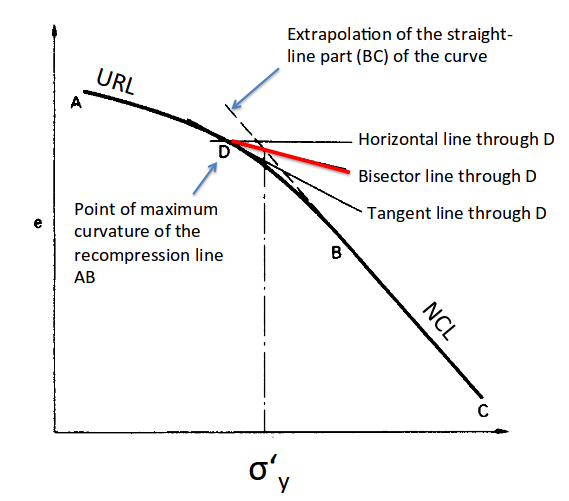
\includegraphics[scale=0.35]{compr_real.png}
\caption{Allure réelle du graphe de $e$ en fonction de $\sigma'$ (échelle logarithmique)}
\label{fig:comprreal}
\end{figure}

Une fois ce point déterminé, si l'on veut calculer un tassement et que l'on se trouve sur une URL, si le sol est préconsolidé, le tassement sera d'abord proportionnel à l'indice de gonflement : $$\frac{s}{H} = \frac{C_S}{1 + e_0}\log\frac{\sigma_f'}{\sigma_0'}$$
Il faut dans un premier temps faire une approximation du tassement pour vérifier si l'on dépasse la contrainte de préconsolidation, c'est-à-dire si l'on revient sur une courbe NCL. Si ce n'est pas le cas, le tassement calculé est correct. Dans l'autre cas, il faut calculer le tassement sur l'URL jusqu'à la contrainte de préconsolidation et ensuite calculer le tassement sur la NCL jusqu'au tassement final : $$\frac{s}{H} = \frac{C_c}{1 + e_0}\log\frac{\sigma_y'}{\sigma_0'} +  \frac{C_S}{1 + e_0}\log\frac{\sigma_f'}{\sigma_y'}$$ où $\sigma_0'$ est la contrainte initiale, $\sigma_y'$ la contrainte de préconsolidation et $\sigma_f'$ la contrainte finale.


\chapter{Résistance au cisaillement et cercle de Mohr}
\section{Rappel : contraintes}
Jusqu'à présent, nous ne nous sommes intéressé uniquement aux contraintes normales. Cependant, si la contrainte n'est pas normale, elle peut se décomposer en une contrainte normale et une contrainte tangentielle (cisaillement). Ceci est représenté à la figure~\ref{fig:shear}.  

\begin{figure}[ht!]
\centering
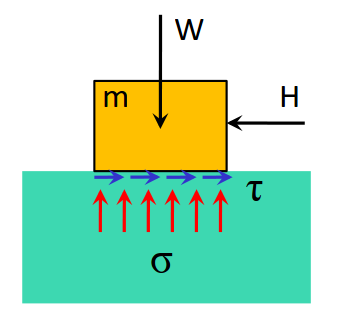
\includegraphics[scale=0.35]{shear.png}
\caption{Contrainte normale et de cisaillement}
\label{fig:shear}
\end{figure}

La contrainte normale est donnée par : $$\sigma = \frac{W}{A}$$ où $W$ est le poids appliqué sur la surface $A$. Par convention, elle est positive en compression.

La contrainte tangentielle est donnée par : $$\tau = \frac{H}{A}$$ où $H$ est la force appliqué parallèlement à $A$. Par convention, elle est positive dans le sens anti-horlogique.

Une contrainte normale produira un changement de taille de l'élément tandis qu'une contrainte de cisaillement provoque un changement de forme. 

Lorsqu'il n'y a pas de contrainte tangentielle, on parle de contrainte principale. Celle-ci s'applique sur une facette principale. En trois dimensions, il y a trois facettes principales mais nous ne nous intéressons ici qu'au cas bidimensionnel. Les contraintes principales sont donc $\sigma_1$ la contrainte principale majeure et $\sigma_3$ la contrainte principale mineure avec $\sigma_1 > \sigma_3$.

\section{Cercle de Mohr}

Lorsque l'on veut déterminer les contraintes sur des plans inclinés de l'élément (figure~\ref{fig:inclinate}), il faut recourir au cercle de Mohr.

\begin{figure}[ht!]
\centering
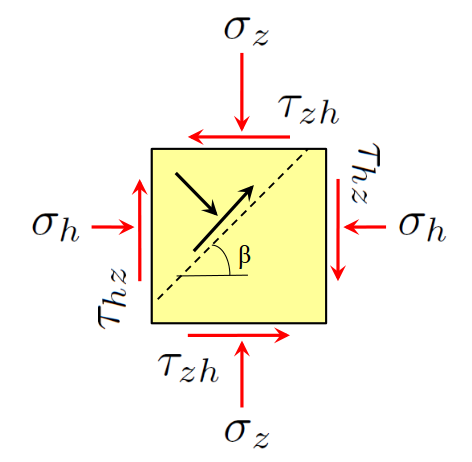
\includegraphics[scale=0.35]{inclinate_plane.png}
\caption{Contraintes sur un cube}
\label{fig:inclinate}
\end{figure}

Pour représenter les contraintes, on utilise un diagramme avec $\sigma$ en abscisses et $\tau$ en ordonnées.
Chaque point du cercle de Mohr (figure~\ref{fig:mohrcircle}) représente les contraintes agissant sur une facette d'orientation quelconque.
\begin{figure}[ht!]
\centering
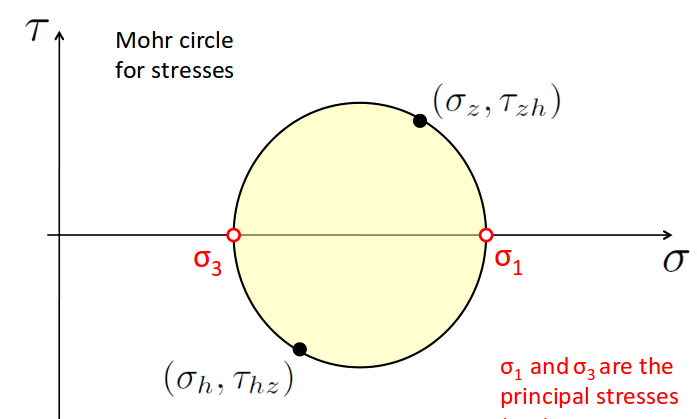
\includegraphics[scale=0.35]{mohr_circle.png}
\caption{Cercle de Mohr}
\label{fig:mohrcircle}
\end{figure}

Si l'on connait les contraintes appliquées sur deux facettes quelconques, il est possible de trouver le cercle de Mohr correspondant en cherchant son centre et son rayon (figure~\ref{fig:mohr2}). Nous avons deux points, donc deux équations. Une bête application de pythagore pour chacun des points donne : $\tau_A^2 + (\sigma_A - C)^2 = R^2$ et $\tau_B^2 + (\sigma_B - C)^2 = R^2$. En soustrayant les deux équations, nous obtenons : $$C = \frac{\tau_A^2 + \sigma_A^2 - \tau_B^2 - \sigma_B^2}{2(\sigma_A - \sigma_B)}$$

\begin{figure}[ht!]
\centering
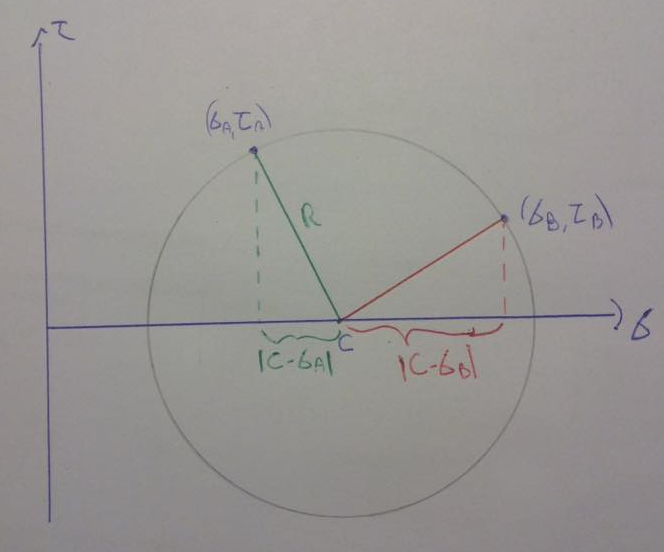
\includegraphics[scale=0.35]{mohr_2.png}
\caption{Détermination du cercle de Mohr}
\label{fig:mohr2}
\end{figure}

A partir de là, il est possible de trouver les contraintes principales mineure et majeure.

\subsection{"Les deux $\theta$"}

Une propriété importante du cercle de Mohr est que si deux facettes forment un angle $\theta$ entre elles, leur rayons dans le cercle de Mohr formeront un angle $2\theta$. Celà permet de trouver facilement les contraintes sur une face si l'on connait l'orientation d'une face sur laquelle s'appliquent des contraintes connues. Ou, dans l'autre sens, celà permet de trouver l'orientation entre deux facettes dont on connait les contraintes. On peut aussi en déduire que deux facettes perpendiculaires entre elles seront diamétralement opposées sur le cercle !

\subsection{Pôle du cercle de Mohr}

Pour trouver les contraintes sur une facette d'orientation quelconque, on peut utiliser la technique du pôle. En supposant le cercle connu ainsi qu'un couple de contraintes s'appliquant sur un plan, il est possible de trouver le pôle du cercle. Pour se faire, il faut tracer une parallèle au plan où la contrainte est appliquée. Le pôle correspond à l'intersection de cette droite et du cercle. Sur la figure~\ref{fig:pole}, les deux couples de points correspondent aux contraintes appliquées conformément à la figure~\ref{fig:inclinate}. La contrainte $\sigma_z$ s'applique bien sur un plan horizontal, le pôle est trouvé en traçant une droite horizontale passant par $\sigma_z$.

\begin{figure}[ht!]
\centering
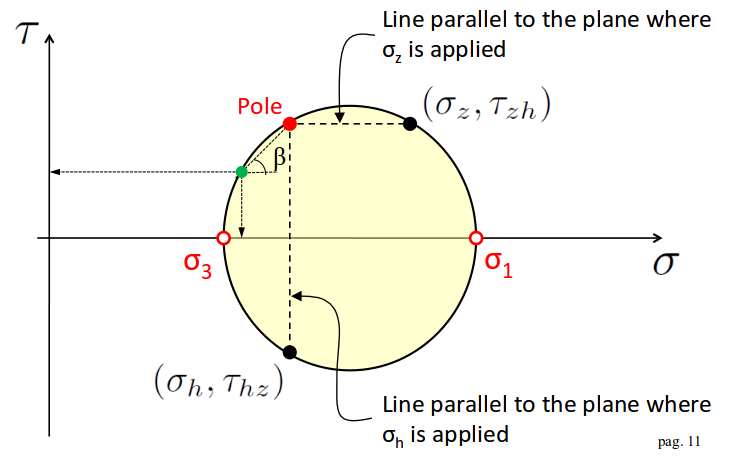
\includegraphics[scale=0.35]{pole.png}
\caption{Pôle du cercle de Mohr}
\label{fig:pole}
\end{figure}

Pour trouver les contraintes s'appliquant sur une facette faisant un angle $\beta$ avec l'horizontale (par exemple), il faut tracer une droite formant un angle avec la droite passant par le pôle et le point d'origine. Sur ce dessin, l'angle $\beta$ est placé comme sur la figure~\ref{fig:inclinate}. Une autre manière de faire aurait été de compter l'angle à partir de la facette du dessus, il vaudrait donc $\pi+\beta$. Il devient donc plus facile de trouver le point voulu en traçant une droite faisant un angle $\pi+\beta$ à partir de a droite reliant le pôle et le point d'orgine $\sigma_z$.

Une fois le point déterminé, des constructions géométriques et trigonométriques permettent de trouver les contraintes voulues.

\subsection{Changement de contraintes}
Si l'on change l'état de contrainte sur l'échantillon, le cercle de Mohr va lui aussi changer, comme illustré à la figure~\ref{fig:morhcght}. 

\begin{figure}[ht!]
\centering
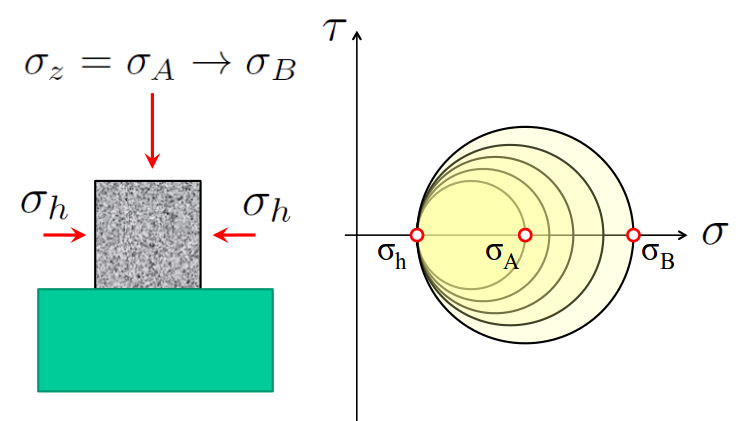
\includegraphics[scale=0.35]{mohr_change.png}
\caption{Evolution du cercle de Mohr}
\label{fig:morhcght}
\end{figure}

En fonction de si l'échantillon est plan ou sphérique, il est possible de représenter ce changement de deux façons différentes, comme le monte la figure~\ref{fig:morhpath}.

\begin{figure}[ht!]
\centering
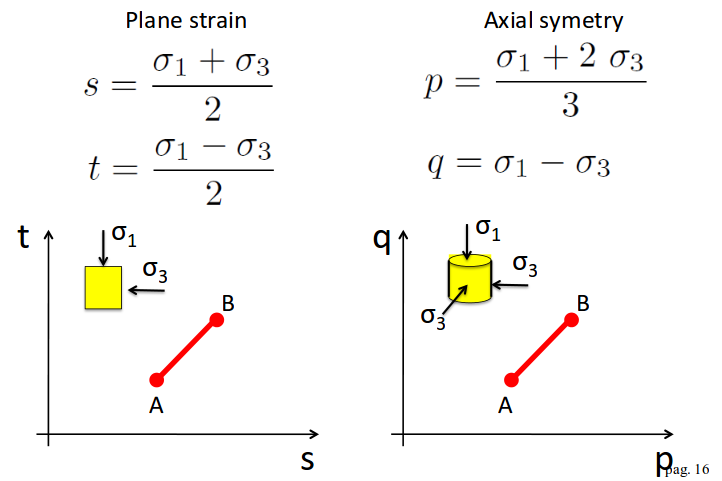
\includegraphics[scale=0.35]{mohr_path.png}
\caption{Représentation des changements d'état}
\label{fig:morhpath}
\end{figure}



\section{Critère de rupture de Mohr-Coulomb}
La rupture d'un sol ne survient pas seulement lorsque la contrainte de cisaillement atteint un maximum, elle survient pour un couple de contraintes $(\sigma, \tau_l)$. Le critère de Mohr-Coulomb définit la courbe intrinsèque (figure~\ref{fig:cohesion}) d'un sol : $$\\tau_l = c + \sigma \tan\phi$$ où $c$ est la cohésion du sol et $\phi$ l'angle de frottement interne.

\begin{figure}[ht!]
\centering
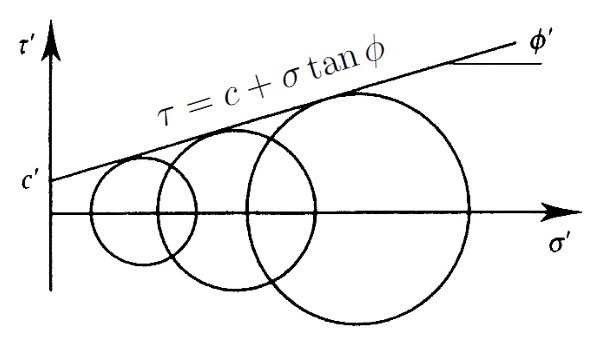
\includegraphics[scale=0.35]{cohesion.png}
\caption{Courbe intrinsèque du sol}
\label{fig:cohesion}
\end{figure}

Lorsque la cohésion est nulle ($c = 0$), le sol est dit \textit{pulvérulent}. L'expression se réduit à : $$\tau_l = \sigma\tan\phi$$ C'est le cas des sables, des graviers.

D'un autre côté, le sol est dit \textit{cohérent}, c'est le cas des argiles. Il est même possible que l'angle de frottement soit nul, auquel cas le sol est dit \textit{purement cohérent}. On obtient : $$\tau_l = c$$

Une méthode pour déterminer la droite intrinsèque est l'essai de la boîte de Casagrande (figure~\ref{fig:casagrande}. 

\begin{figure}[ht!]
\centering
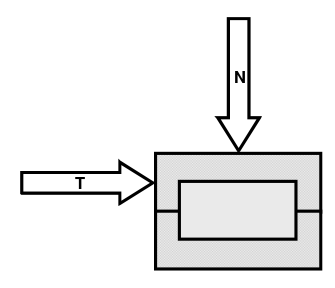
\includegraphics[scale=0.35]{casagrande.png}
\caption{Boîte de Casagrande}
\label{fig:casagrande}
\end{figure}

La contraintre normale est : $$\sigma = \frac{N}{\Omega}$$ et la contrainte de cisaillement est : $$\tau = \frac{T}{\Omega}$$ où $\Omega$ est la section de l'échantillon.

Pour une contrainte normale donnée, on augmente la contrainte de cisaillement jusqu'à obtenir la rupture de l'échantillon. Le test est effectué sur au moins trois échantillons soumis à des efforts normaux différents et on en déduit la droite intrinsèque.

La déformation liée à la contrainte de cisaillement est différente si l'eau peut drainer à travers le sol ou non. la figure~\ref{fig:drained} représente la courbe intrinsèque si le sol peut éjecter/capter l'eau à travers ses pores. Dans le cas contraire (figure~\ref{fig:undrained}), le sol ne peut pas éjecter d'eau de ses pores, son volume reste donc constant. En conséquence, la contrainte apparente ne change pas (la pression interstitielle change), et la contrainte de cisaillement ne change pas même si la contrainte normale augmente.

\begin{figure}[ht]
\begin{subfigure}[h!]{0.45\textwidth}
\centering
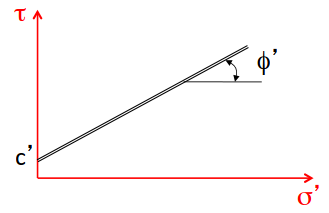
\includegraphics[scale=0.40]{drained.png}
\caption{Avec drainage}
\label{fig:drained}
\end{subfigure}
\begin{subfigure}[h!]{0.45\textwidth}
\centering
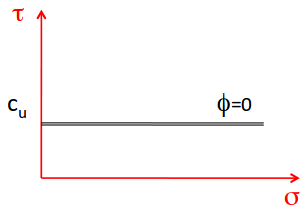
\includegraphics[scale=0.42]{undrained.png}
\caption{Sans drainage}
\label{fig:undrained}
\end{subfigure}
\caption{Cisaillement en fonction de l'effort normal}
\end{figure}

\part{}

\chapter{Les roches et les sols}

\section{Origines et classification des sols}
Tout ce qui concerne la formation, classification des sols/roches se retrouve au chapitre~\ref{sols}.
\bigbreak

\section{Caractéristiques physiques et techniques des roches et sols}
\subsection{Porosité} Dans une roche, la matière minérale ne remplit pas tout l'espace, il existe des vides formés par des fissures ou des pores. La proportion de vides est appelée porosité. La \textit{porosité totale} correspond au rapport entre le volume de vides et le volume total de la roche. La \textit{porosité ouverte} quant à elle est déterminée par la proportion de vides reliés entre eux, reliés à l'eau. C'est elle qui conditionne la perméabilité d'un matériau, sa capacité à laisser circuler l'eau. Si nous nous rappelons la loi de Darcy : $v = k i$, nous pouvons définir une nouvelle vitesse, la vitesse convective : $v_c = \frac{\text{vitesse de Darcy}}{\text{porosité efficace}}$. Le tableau~\ref{porosity} reprend la porosité de certains matériaux types.

\begin{figure}[ht]
\centering
\begin{tabular}{|c|c|c|c|c|c|c|c|c|c|}
\hline 
&\textbf{Roche} & \textbf{Sol} & \textbf{Béton} & \textbf{Acier} & \textbf{Verre} & \textbf{Al} & \textbf{Maçonnerie} & \textbf{MDF} & \textbf{Lamellé/collé} \\ 
\hline 
\textbf{Porosité} & $1-50\%$ & $40-80\%$ & $20\%$ & $<1\%$ & $<1\%$ & $<1\%$ & $20-50\%$ & $80\%$ & $60-80\%$ \\ 
\hline 
\end{tabular} 
\caption{Porosité}
\label{porosity}
\end{figure}

La détermination en laboratoire de la porosité totale se faut soit au pycnomètre, soit au mercure : on mesure la quantité de mercure pouvant être insérée dans le solide à différentes pressions. Pour la porosité efficace, on mesure simplement le volume d'eau dans un échantillon à saturation.

\subsection{Masse volumique $\rho$} Encore une fois, on distngue deux types de masse volumique, la masse volumique réelle qui est le rapport entre la masse de solide et le volume réel occupé par celui-ci (en relation avec le poids spécifique des molécules $\gamma_s$) ainsi que la masse volumique apparente, rapport entre la masse de solide et le volume apparent occupé par celui-ci (en relation avec le poids volumique $\gamma$). Le tableau~\ref{massevolumique} reprend quelques masses volumiques caractéristiques.

\begin{figure}[ht]
\centering
\begin{tabular}{|c|c|c|c|c|c|c|c|c|c|c|}
\hline 
&\textbf{Roche} & \textbf{Sol} & \textbf{Béton} & \textbf{Acier} & \textbf{Verre} & \textbf{Al} & \textbf{Maçonnerie} & \textbf{MDF} & \textbf{Lamellé/collé} & \textbf{Mercure}\\ 
\hline 
\textbf{$\rho~[\unit{\gram\per\centi\cubic\meter}]$} & 0.9-3.5 & 1.2 & 2.2 & 7.5 & 2.53 & 2.7 & 2 & 0.8 & 0.38 &  13 \\ 
\hline 
\end{tabular} 
\caption{Masse volumique}
\label{massevolumique}
\end{figure}

La détermination en laboratoire de la masse volumique apparente se fait à partir d'échantillons remaniés (broyés) dont on mesure la masse. On les sature ensuite pour déterminer le volume de vides afin de trouver le volume réel occupé par le solide. Ceci se fait par exemple au pycnomètre. Pour déterminer la masse volumique réelle, on utilise des échantillons non remaniés.

\subsection{Coefficient d'absorption d'eau} L'absorption d'eau correspond à la capacité d'une roche à capter de l'eau dans ses pores. Il est important d'avoir une connaissance de cette caractéristique si l'ouvrage est susceptible d'entrer en contact avec l'eau. L'absorption d'eau provoque des problèmes de stabilité (gonflements/tassements). 

L'\textit{absorption d'eau par capillarité} reflète la quantité d'eau pouvant être captée par le solide par capillarité, avec une seule face en contact d'eau. Elle s'exprime par le coefficient de capillarité, exprimé en \unit{\gram\per(\meter\squared\usk\power{s}{\frac{1}{2}})}. Le tableau~\ref{capillarity} reprend des coefficients de capillarité pour des matériaux types.

\begin{figure}[ht]
\centering
\begin{tabular}{|c|c|c|c|}
\hline 
 & \textbf{Roche} & \textbf{Béton} & \textbf{Maçonnerie} \\ 
\hline 
\textbf{Coefficient de capillarité [\unit{\gram\per(\meter\squared\usk\power{s}{\frac{1}{2}})}]} & 10-80 & 1 & 5-15 \\ 
\hline 
\end{tabular} 
\caption{Coefficient de capillarité}
\label{capillarity}
\end{figure}

Pour déterminer ce coefficient, on place un matériau séché en contact avec de l'eau par une seule de ses parois. L'évolution de la masse et reportée sur un graphique en $\sqrt{t}$ et le coefficient d'absorption d'eau par capillarité peut être calculé.
\bigbreak

L'eau peut aussi être absorbée lorsque le matériau est totalement immergé. Cette caractéristique correspond donc à la masse d'eau pouvant être absorbée lorsque le solide est complétement immergé et s'exprime en pourcentage de masse. Les argiles et les tourbes sont des matériaux gonflants.

La méthode d'essai consiste à plonger le matériau séché pendant \unit{48}{\hour}, le peser et le replonger par phases de \unit{14}{\hour} jusqu'à obtention d'une masse constante.

\subsection{Perméabilité $k$}
Le coefficient de perméabilité découle directement de la loi de Darcy. L'essai de perméabilité peut être réalisé à charge constante ou variable. Le chapitre~\ref{chap:k} explique en détail la détermination de ce coefficient. Le tableau~\ref{permebility} reprend des valeurs caractéristiques pour différents types de sols.

\begin{figure}[ht]
\centering
\begin{tabular}{|c|c|c|c|}
\hline 
 & \textbf{Argile} & \textbf{Limon} & \textbf{Sable} \\ 
\hline 
\textbf{$k [\unit{\meter\per\second}]$} & $\power{10}{-8}$ & $\power{10}{-6}-\power{10}{-7}$ & $\power{10}{-3}$ \\ 
\hline 
\end{tabular} 
\caption{Coefficient de perméabilité}
\label{permebility}
\end{figure}


\subsection{Résistance à la compression uniaxiale $R_c$} Il s'agit de la contrainte maximale (mesurée en \unit{\mega\pascal}) supportée par la roche lors d'un essai à chargement monotone croissant selon une direction.
Lors du test, il est possible de caractériser le comportement (figure~\ref{fig:déf}) de la roche selon son mode de déformation et de rupture, dépendant du type de sol ainsi que des conditions d'essai.

\begin{figure}[ht!]
\centering
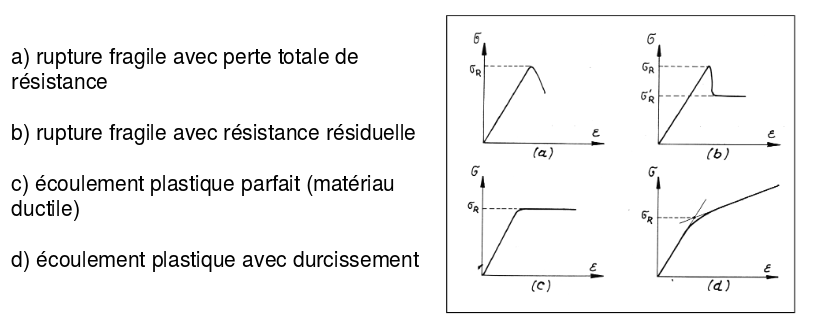
\includegraphics[scale=0.45]{res.png}
\caption{Différents modes de rupture}
\label{fig:déf}
\end{figure}

La figure~\ref{compr} reprend des valeurs types pour certains matériaux.

\begin{figure}[ht]
\centering
\begin{tabular}{|c|c|c|c|c|c|c|c|c|c|}
\hline 
&\textbf{Roche} & \textbf{Sol} & \textbf{Béton} & \textbf{Acier} & \textbf{Verre} & \textbf{Al} & \textbf{Maçonnerie} & \textbf{MDF} & \textbf{Lamellé/collé} \\ 
\hline 
\textbf{$R_c~[\unit{\mega\pascal}]$} & 6-200 & 0.1-1 & 50 & 180-1000 & 1000 & 250 & 2.5-20 & 10-15 & 24-32 \\ 
\hline 
\end{tabular} 
\caption{Résistance à la compression}
\label{compr}
\end{figure}

Pour déterminer cette caractéristique, le test est simple : compression progressive d'un échantillon cylindrique jusquà la rupture.

Un autre essai utilisé est l'essai à l'\oe{}domètre (voir chapitre~\ref{chap:compr}). L'échantillon est soumis à une compression et le dispositif permet l'évacuation de l'eau interstitielle. La compression est mesurée en fonction du temps.

\subsection{Résistance au cisaillement} Le cisaillement correspond à l'application de deux forces de sens opposé et décalées l'une par rapport à l'autre. Comme pour la compression, on peut caracrtériser le matériau en fonction de son mode de déformation/rupture (figure~\ref{fig:déf}).

La méthode de détermination est très simple : l'échantillon est placé dans une boite de cisaillement constituée de deux parties séparées dans un plan horizontal, suivant lequel le cisaillement est imposé.

\subsection{Résistance aux chocs} Elle est appelée résilience et correspond à la capacité d'un matériau à absorber l'énergie sous l'effet d'un choc. Elle s'exprime en \unit{\joule}.

Le premier test est le test au scléromètre (marteau Schmidt) qui consiste à cogner le matériau avec le scléromètre qui mesure automatiquement l'énergie absorbée/renvoyée par la matériau.

Le deuxième test est réalisé avec le \textit{Mouton Charpy} et mesure l'énergie nécessaire pour rompre en un choc l'échantillon. Le mouton est lâché d'une certaine hauteur, percute l'échantillon préalablement entaillé et remonte jusqu'à une hauteur plus faible. L'énergie peut donc être calculée en fonction la hauteur d'arrivée du mouton.

\subsection{Résistance à l'abrasion} Ceci correspond à la résistance d'un matériau face à un forttement mécanique. Cette grandeur est quantifiée par le coeffient d'abrasivité qui correspond au rapport entre la puissance absorbée par la destruction de la roche et la puissance absorbée par l'usure du taillant. 

Pour tester cette caractéristique, on utilise des appareils appliquant une abrasion (le plus souvent circulaire) à pression constante et mesurant la perte de masse de l'échantillon.

\subsection{Dureté} La dureté est plus un concept qu'une propriété et correspond à la capacité d'un matériau à s'opposer à la pénétration d'une pointe. L'échelle de Mohs définit la dureté en fonction des matériaux (figure~\ref{fig:mohs}). 

\begin{figure}[ht!]
\centering
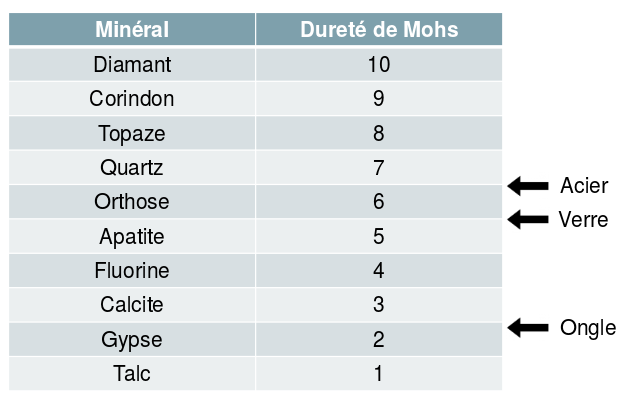
\includegraphics[scale=0.45]{mohs.png}
\caption{Echelle de Mohs}
\label{fig:mohs}
\end{figure}

L'échelle de Mohs est pratique pour avoir une idée rapide de la dureté d'un matérieux. En effet, en dessous de 2, il est possible de griffer la pierre avec un ongle. En dessous de 5.5-6, le verre griffera la pierre tandis qu'au dessus de cette valeur, le verre se fera griffer.

\subsection{Gelivité} Permet de qualifier la détérioration d'une roche sous l'action du gel. Une pierre est dite gelive si elle absorbe l'humidité et, lors du gel, se solidifie et augmente de volume, pouvant engendrer des fissures (on parle alors de \textit{gélifraction} ou \textit{cryoclastie}).

La gelivité dépend de la capacité de la roche à absorber l'humidité, de la dureté et des conditions envronnementales. L'essai de gélivité consiste à appliquer des cylces de gel/dégel jusqu'à rupture du matériau (taux d'humidité et dimensions de l'échantillon normés).

\subsection{Conductivité thermique $\lambda$} Représente l'énergie transférée par unité de surface et de temps sous un gradient de température de 1 Kelvin par mètre. Elle est mesurée en \unit{\watt\per\meter\usk\kelvin}. Des valeurs caractéristiques sont reprises à la figure~\ref{cond}.

\begin{figure}[ht]
\centering
\begin{tabular}{|c|c|c|c|c|c|c|c|c|c|}
\hline 
&\textbf{Roche} & \textbf{Sol} & \textbf{Béton} & \textbf{Acier} & \textbf{Verre} & \textbf{Al} & \textbf{Maçonnerie} & \textbf{MDF} & \textbf{Lamellé/collé} \\ 
\hline 
\textbf{$\lambda~[\unit{\watt\per\meter\usk\kelvin}]$} & 3 & 0.3-0.6 & 1-2 & 50 & 1 & 160 & 0.2-0.8 & 0.15 & 0.1-0.2 \\ 
\hline 
\end{tabular} 
\caption{Conductivité thermique}
\label{cond}
\end{figure}

La conductivité thermique se mesure dans des conditions adiabatiques en faisant passer un flux thermique $Q$ dans l'échantillon de section $A$ et la chaleur dissipée est récupérée dans un bain thermique de l'autre côté de l'échantillon. Des capteurs séparés d'une distance $L$ mesurent la différence de température $\Delta T$ dans l'échantillon. La conductivité thermique est alors donnée par : $$\lambda = \frac{Q L}{A \Delta T}$$

Une autre méthode consiste à chauffer une face d'un échantillon et mesurer la température de la face arrière par infrarouges. Le temps nécesaire pour que la face arrière atteignent la moitié de la température de l'échantillon permet de calculer la conductivité thermique.

La figure~\ref{fig:cond_2} donne d'autres valeurs importantes.

\begin{figure}[ht!]
\centering
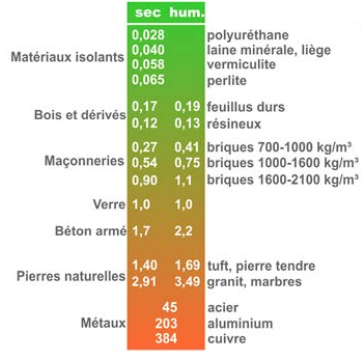
\includegraphics[scale=0.45]{cond_2.png}
\caption{Conductivité thermique}
\label{fig:cond_2}
\end{figure}

\chapter{Méthodes d'investigation \textit{in-situ}}

\section{Eléments de base d'une campagne de caractérisation géologique/géotechnique}
Le sol est un matériau naturel dont les caractéristiques sont fort variable d'un point à l'autre, on ne contrôle pas leur propriétés, il faut donc s'adapter et étudier préalablement le terrain. Plus l'étude de terrain sera poussée, plus les risques d'imprévus sont réduits. Les fondations sont les éléments principaux en contact avec le sol, il est donc fondamental qu'elles soient bien réalisées.

Différents critères doivent être pris en compte afin de bien réalisé les fondations d'un ouvrage : 
\begin{itemize}
\item la capacité portante du sol;
\item les tassements, pour assurer que l'ouvrage ne soit pas endommager par les mouvements du sol;
\item les effets de l'ouvrage sur le sol existant, et
\item le niveau de la surface piézométrique qui peut influer sur la stabilité des fondations.
\end{itemize}

L'étude comprend plusieurs phases : 
\begin{itemize}
\item étude de faisabilité, incluant une étude (hydro-)géologique, économique, technique et bibliographie;
\item détermination de propriétés physiques et mécaniques pour évaluer le comportement des sols sous l'ouvrage futur;
\item détermination de la surface piézométrique par étude hydrogéologique, et
\item suivi et réception technique des travaux requis, pour s'assure le respect du cahier des charges, le respect de l'environnement, et pour pouvoir s'adapter si des conditions changent ou si de nouvelles connaissances/contraintes apparaissent.
\end{itemize}

Toute construction présente des risques, ceux-ci doivent tous être pris en compte : risques liés à la santé et la sécurité (glissement de terrain,...), risques d'infiltration d'eau, risques liés à l'environnement (nappes et sols contaminés), risques liés à la qualité de l'ouvrage, risques de délais de construction et risques financiers.

Quelques exemples de problèmes géotechniques sont : glissement de terrain, gonflement des argiles, tassement du sol, construction à la limite de nappe phréatique (risque d'inondation),...

\section{Forages}
Les forages sont destinés à valider les hypothèses de terrain, la géophysique, et à contrôler la qualité chimique ainsi que les propriétés mécaniques. Cependant les forages coûtent cher et ne fournissent que des données ponctuelles. Il faut donc implanter judicieusement le forage et stocker les échantillons. Les techniques de forage dépendent de la nature du terrain.

\subsection{Terrains meubles}
Il existe des méthodes différentes si le sol est constitué d'argiles ou des sables/graviers (si le sol est cohésif ou non). Le forage est accompagné d'un tubage pour éviter l'effondrement des parois. L'usage d'un carottier double paroi (ou simples pour les sédiments cohésifs) permet le prélèvement d'échantillons non remaniés (ou peu remaniés). 

Les forages à tarière hélicoïdale (sol cohésif, figure~\ref{fig:helico}) ou à cuillère à clapet (sables, graviers) entrainent un remaniement important.

\begin{figure}[ht]
\centering
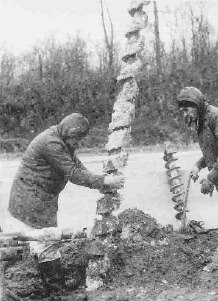
\includegraphics[scale=0.6]{tariere.png}
\caption{Tarière hélicoïdale}
\label{fig:helico}
\end{figure}

\subsection{Terrains rocheux durs}
Ces forages sont effectués avec une injection d'eau et d'additifs. Ils peuvent être carottés ou destructifs. 

Les forages destructifs (figure~\ref{fig:destr}) remontent des débris (\textit{cuttings}) et sont effectués avec un outil qui peut prendre différentes formes. Les dents sont faites dans un matériau très dur (selon l'échelle de Mohs) tel que le diamant. Par rotation, percussion et pression, l'outil attaque la roche et de l'eau sous pression fait remonter les cuttings à la surface. Le forage est tubé au fur et à mesure. Cette technique est rapide et bon marché.


\begin{figure}[ht!]
\begin{subfigure}[h!]{0.45\textwidth}
\centering
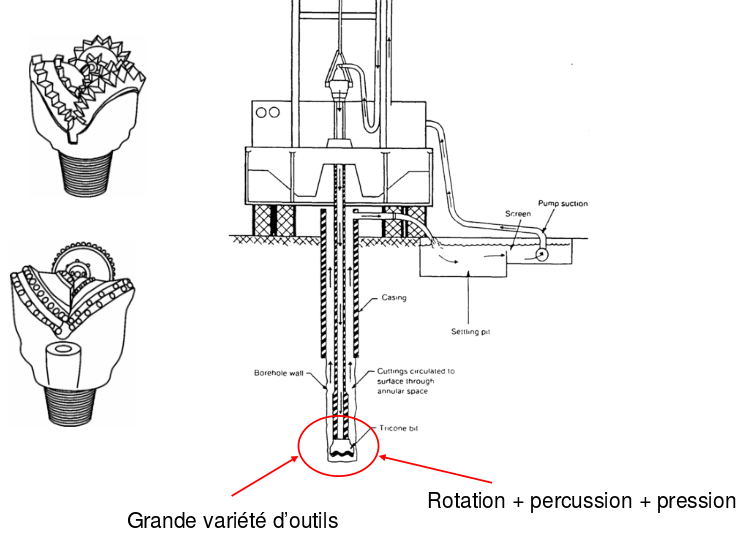
\includegraphics[scale=0.30]{forage_destr.png}
\caption{Forage destructif}
\label{fig:destr}
\end{subfigure}
\begin{subfigure}[h!]{0.45\textwidth}
\centering
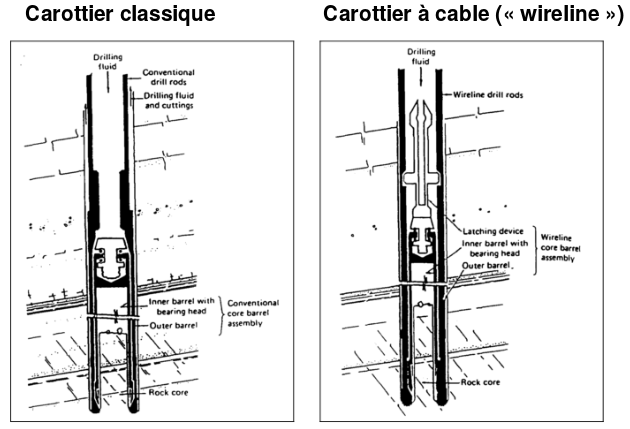
\includegraphics[scale=0.30]{forage_carotte.png}
\caption{Carottiers}
\label{fig:carotte}
\end{subfigure} 	
\caption{Forages}
\end{figure}

Les forages carottés (figure~\ref{fig:carotte}) remontent un cylindre de roche, permettent un échantillonage précis et donnent une bonne information lithographique mais sont relativement lents et coûteux. 

Les carottiers sont constitués d'un cylindre au au bout duquel sont fixés des dents de diamant. Le forage est réalisé par la rotation de celui-ci.

Les résultats d'un carottage sont minutieusement stocké par ordre de sortie et l'on peut définir un taux de récupération total, TRT (figure~\ref{fig:tauxrecuperationtotal}). Celui-ci est le rapport entre la longueur cumulée des carottes et la longueur forée. Cela reflète la compacit du massif mais aussi la qualité technique du forage. Idéalement il doit être supérieur à 90\% et il y a des pénalité (de payement) si il est inférieur à 80\%.

\begin{figure}[ht!]
\begin{subfigure}[h!]{0.45\textwidth}
\centering
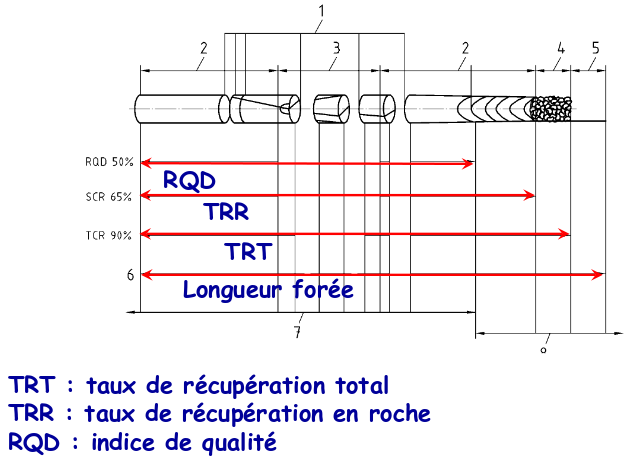
\includegraphics[scale=0.30]{taux_recup.png}
\caption{Taux de récupération}
\label{fig:tauxrecuperationtotal}
\end{subfigure}
\begin{subfigure}[h!]{0.45\textwidth}
\centering
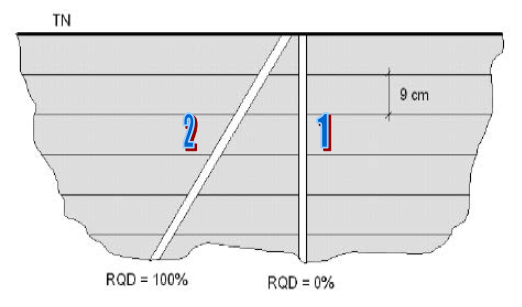
\includegraphics[scale=0.30]{rqd.png}
\caption{Application du RQD}
\label{fig:rqd}
\end{subfigure}
\caption{Résultat d'un carottage}
\end{figure}

Une autre information donnée par le forage est l'indice de qualité RQD (\textit{Rock Quality Designation}). Celui-ci est la rapport de la somme des carottes de plus de \unit{10}{\centi\meter} de longs et de la longueur totale de forage. Celui-ci est exprimé en \% (tableau~\ref{rqd2}). 

\begin{figure}[ht!]
\centering
\begin{tabular}{|c|c|c|c|c|c|}
\hline 
\textbf{RQD} & 0-25\% & 25-50\% & 50-75\% & 75-90\% & 90-100\% \\ 
\hline 
\textbf{Qualité} & Très faible & Faible & Correcte & Bonne & Excellente \\ 
\hline 
\end{tabular} 
\caption{RQD}
\label{rqd2}
\end{figure}

Cependant, il faut faire attention, dans certains cas, le RQD peut varier en fonction de l'orientation de forage comme le montre la figure~\ref{fig:rqd}. En effet, le RQD est de 0 si l'on fore verticalement et il est de 100\% si l'on fore en oblique.

\bigbreak
Il existe aussi d'autres méthodes de forage tels que	le forage à 90\unit{degree} par rapport aux couches du sol ou des forages horizontaux.

De plus, lors de certains forage, une diagraphie est réalisée. Il s'agit de sondes qui mesurent les caractéristiques des roches traversées lors d'un forage.


\section{Prospection géophysiques}

Ce type d'analyse du sol fait appel aux propriétés physiques des terrains : résistivité, vitesse de propagation/réfraction des ondes,... Ce sont des méthodes de surface, donc non destructrices et l'information récoltée n'est pas ponctuelle, le coût est donc réduit.

\subsection{Sismique réfraction}
Une onde est produite en un point du sol et est captée par différents géophones (figure~\ref{fig:sism}). Etant donné que la vitesse de propagation change d'un milieu à l'autre, il est possible de déterminer les épaisseurs des différentes couches du sol, la transition sol/roche, de déterminer la présence de failles et poches karstiques. La profondeur d'application est de \unit{40}{\meter}. 

\begin{figure}[ht]
\centering
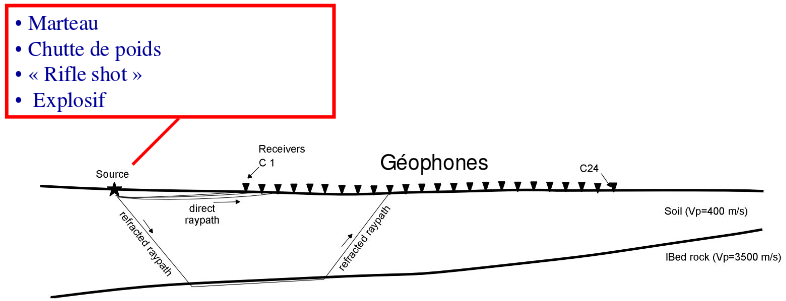
\includegraphics[scale=0.5]{sismique_refraction.png}
\caption{Sismique réfraction}
\label{fig:sism}
\end{figure}

Un détail important est que les vitesses de propagation doivent augmenter avec la profondeur. Les vitesses de propagation $v_p$ pour différentes couches du sol sont données à la figure~\ref{tab:speed}.

\begin{figure}[ht!]
\centering
\begin{tabular}{|c|c|c|c|c|c|c|}
\hline 
\textbf{Type de sol/roche} & Sol (surface) & Sol (sable, argile,...) & Eau & Roches fracturées & Roche & Acier \\ 
\hline 
\textbf{$v_p [\unit{\meter\per\second}]$} & 150-300 & 300-800 & 1500 & 2000-2500 & >3500 & 5000-5500 \\ 
\hline 
\end{tabular} 
\caption{Vitesses de propagation}
\label{tab:speed}
\end{figure}

Cette technique permet de classifier les terrains à excaver en trois catégorie : 
\begin{itemize}
\item meuble : pelle mécanique
\item rippable : terrain rocheux peu compact, ripper (déconsolider à l'aide d'une dent)
\item compact : abattage à l'explosif
\end{itemize}

\subsection{Tomographie électrique}
Cette technique consiste à injecter un courant continu par des électrodes d'émission et à mesurer une différence de potentiel grâce à des électrodes de réception (figure~\ref{fig:tomo}).

\begin{figure}[ht]
\centering
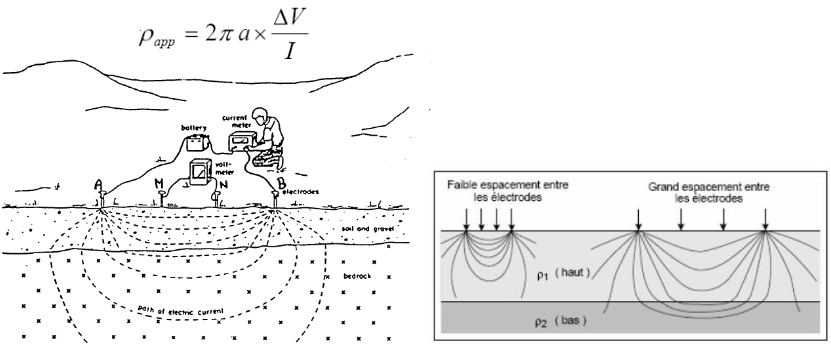
\includegraphics[scale=0.5]{tomographie.png}
\caption{Tomographie électrique}
\label{fig:tomo}
\end{figure}

On peut alors déduire la résistivité électrique du terrain à une certaine profondeur par la loi d'Ohm. Il est donc possible de déterminer l'épaisseur de la couverture meuble et la transition sol/roche, l'emplacement de failles et poches karstiques. La profondeur d'investigation va jusque \unit{50}{\meter}, cependant la résolution diminue avec la profondeur. 

Le tableau~\ref{resistivity} reprend des valeurs de résistivité pour différents types de sols.

\begin{figure}
\centering
\begin{tabular}{|c|c|c|c|c|c|}
\hline 
\textbf{Type de sol/roche} & Sol argileux & Sable & Graviers & Roche fracturée & Roche compacte \\ 
\hline 
\textbf{Résistivité [\unit{\ohm\usk\meter}]} & 10-30 & 50-200 & 200-400 & 300-1000 & \power{10}{3}-\power{10}{6} \\ 
\hline 
\end{tabular} 
\caption{Résistivité des sols}
\label{resistivity}
\end{figure}


\section{Méthodes d'investigation invasives}

\subsection{Essai au pénétromètre dynamique}
Cet essai est utilisé au stade préliminaire ou en complément d'autres essais et consiste à enfoncer dans le sol un train de tiges muni d'une pointe à l'extrémité. Le nombre de coups nécessaires à un certain enfoncement permet de déduire la résistance de pointe du sol. 
\paragraph*{Type A} Injection de boues de forage, permet d'évaluer la capacité portante d'un sol.
\paragraph*{Type B} Pas d'injection de boues, sondage limité en profondeur, souvent associé à d'autres essais pour vérifier l'homogénéité d'un site.
\paragraph*{Type Panda} Portatif, coups à la main, pour le contrôle de compactage des tranchées ou remblais, pour les zones d'accès difficile. Limité à \unit{3}{m} de profondeur.
\paragraph*{Au carottier} Peu utilisé, battage d'un carottier, convient aux sols fins et grenus.

\subsection{Essai CPT (Cone Penetration Test)}
Essai de pénétration statique, c'est une méthode d'investigation de qualité. Le test consite à enfoncer par effort progressif une tige équipée d'une pointe dans le sol à l'aide d'un vérin hydraulique et mesurer l'effort requis pour un certain enfoncement. Le frottement latéral ainsi que la résistance à la pointe sont mesurés. 

L'essai est discontinu, la pointe seule est enfoncée à vitesse constante (\unit{2}{\meter\per\second}) sur une certaine distance. On mesure donc la résistance à la pointe. Ensuite, le tube est poussé et rattrape la pointe et le frottement latéral peut donc être mesuré ainsi que l'effort total, somme des deux mesures précédentes. L'opération est répétée tous les \unit{20}{\centi\meter}. Un autre essai existe, l'essai à la pointe électrique donne, lui, des mesures continues.

Le frottement latéral permet de déterminer la nature d'un sol : les argiles ont un frottement latéral élevé tandis qu'il est faible pour les sables. La mise en graphe des résultats permet de déterminer la cohésion et l'angle de frottement du sol.

La mise en \oe{}vre de ce test nécessite de lester l'appareil ou de l'ancrer dans le sol. L'appareil est souvent mis en place sur un véhicule lourd (15-25 tonnes), rendant la mise en place facile.

Le principal inconvénient est la non représentativité de l'essai, si un point dur est rencontré, il amènera à de mauvais paramètres. En fonction du matériel choisi pour fixer l'appareil, le refus sera parfois obtenu avant la profondeur projetée minimale d'investigation.

\subsection{Essai pressiométrique} 
Ce test mesure la déformabilité et la résistance à la rupture du sol. Une sonde est descendue dans un forage de même diamètre et un liquide incompressible gonfle la sonde, déformant le sol. La variation de volume de la sonde ainsi que la pression appliquée permet de mesurer la déformation du sol. La pression augmente par paliers et est répétée tous les 1.5-2 mètres. 

Cet essai est praticable pour tous les types de sols et roches et est le seul essai à fournir à la fois un critère de déformabilité et de rupture.

\subsection{Essai phicométrique} 
Equivalent \textit{in-situ} de l'essai triaxial permettant de mesurer la cohésion et l'angle de frottement, utilisé pour les échantillons difficilement prélevables sans remaniement. Une sonde est placée dans forage de diamètre calibré, en la gonflant des dents sortent et se fixent sur les parois. La sonde est tirée vers le haut. Le test est refait en gonflant plus la sonde et à profondeurs différentes. Nécessite un essai pressiométrique préalable pour connaître la pression à appliquer et ne convient pas pour les sols très mous/grossiers ou dans la roche.

\subsection{Essai scissométrique}
Permet de mesurer la cohésion du sol, par cisaillement direct et est adapté aux sols fins cohérents saturés de faible résistance, ne convient pas aux sables lâches. Un appareil muni de 4 pales est enfoncé dans le sol et mis en rotation. La rotation cisaille le sol sur une surface cylindrique. La mise en graphique de la force nécessaire en fonction de la rotation permet de déterminer la résistance maximale au cisaillement (cohésion scissométrique) et la résistance après perte de la cohésion initiale (cohésion remaniée).

\subsection{Essai de pression/perméabilité}
Cet essai permet de déterminer la possibilité de circulation d'eau dans le sol. Un obturateur est placé dans un forage à profondeur souhaitée et de l'eau est injectée sous pression en dessous de l'obturateur. Le débit d'injection est mesuré pour différentes pressions. Ce test s'applique à la plupart des roches et sols capable de supporter la pression maximale d'injection (\unit{1}{\mega\pascal}), ne convient pas aux sols meubles. Facile à mettre en oeuvre, permet d'identifier les hétérogénéités de perméabilité dans le sol.


\chapter{Géoressources en eau}

\section{Exploitation de l'eau}
\paragraph*{Remarque} Les notions d'aquifère, aquitard et aquiclude sont définies au chapitre~\ref{chap:eau}
\bigbreak

\subsection{Lithologies rencontrées}
\paragraph*{Aquifère} Les aquifères peuvent être constitués de calcaire, grès ou sables. Les calcaires ne sont pas poreux mais présentes de nombreuses fractures à travers lesquelles l'eau peut circuler. Les grès ont une perméabilité essentiellement de fracture mais aussi grâce à la porosité. Les sables présentent une perméabilité de pores, plus les grains sont gros, plus l'écoulement est facilité.
\paragraph*{Aquitard} Ceux-ci sont principalement constitués d'argiles sableux peu perméables.
\paragraph*{Aquiclude} Ils sont formés de shales, schistes, argiles, silts imperméables.

\subsection{Puits}
L'eau souterraine est généralement puisée dans l'aquifère directement par un puits.

\subsection{Barrages}
Les barrages permettent de stocker une importante quantité d'eau de surface. L'eau doit être traitée pour être rendue potable.

\subsection{Emergence}
Cette technique profite directement de l'émergence naturelle de l'eau. Celle-ci doit être traitée.

\subsection{Drains et galeries}
Ce sont des tubes perméables dont le rôle est de drainer l'eau.

\subsection{Carrières} 
Tout au long de l'exploitation d'une carrière, celle-ci s'agrandit et s'approfondit, jusqu'à un point où le niveau est en dessous du niveau de la nappe souterraine. Des venues d'eau apparaissent, il faut donc l'évacuer, cette opération s'appelle l'\textit{exhaure}. Cette eau était généralement rejetée dans un cours d'eau et ce n'est que récemment qu'elle est mise en valeur en la potabilisant.

\section{Mesures de protection}

Les captages d'eau sont en permanence soumis à des risques de pollution. Afin de les protéger, des zones de prévention sont établies tout autour. Ces zones sont définies par différentes études (hydro-)géologiques, géophysiques, d'essais de traçage et de modélisation.

Il existe trois zones de prévention (figure~\ref{fig:zonesprevention}) définies par le temps qu'un polluant mettrait pour atteindre le captage.

\begin{figure}[ht]
\centering
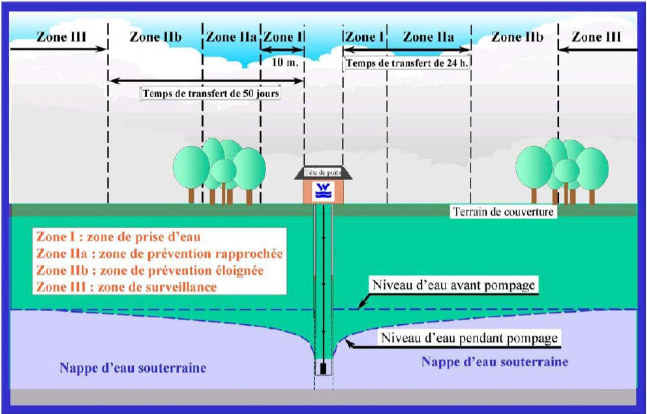
\includegraphics[scale=0.5]{zone_prevention.png}
\caption{Zones de prévention}
\label{fig:zonesprevention}
\end{figure}

\subsection{Zone I : zone de prise d'eau}
Celle-ci est située dans un rayon de 10 mètres autour des installations du captage. Cette zone appartient au producteur d'eau et aucune activité autre que la production d'eau n'est autorisée.

\subsection{Zone IIa : zone de prévention rapprochée}
A l'intérieur de cette zone, une pollution transportée par les eaux souterraines atteindrait le captage en 24 heures.

Dans cette zone, certaines activités sont interdites : stockage enterrés d'hydrocarbures, engrais ou pesticides, les lieux de concentration permanente d'animaux, les terrains de camping,...

Dans cette zone, certaines activités sont réglementées : enclos couverts pour animaux, l'épandage de fertilisant/pesticides, forages,...

\subsection{Zone IIb : zone de prévention éloignée}
Dans cette zone, un polluant atteint le captage en une durée de 1 à 5 jours. 

Dans cette zone, certaines activités sont interdites : puits perdants, nouveau cimetières, nouveaux campings,...

Dans cette zone, certaines activités sont réglementées :  stockage d'engrais/pesticides, installation de valorisation/élimination des déchets,...

\subsection{Le code de l'eau et le décret sol}
Le code de l'eau reprend toutes les législations dans le domaine de l'eau. Il est constamment actualisé en fonction des nouvelles connaissances, techniques.
\bigbreak

Le décret sol vise à prevenir la pollution du sol, à organiser les investigations pour établir l'existence d'une pollution et détermine les modalités d'assainissement.

Différentes valeurs caractérisent la concentration en polluant dans le sol.

\paragraph*{Valeur de référence} Valeur des concentrations attendues dans le sol en l'absence de variations géologiques et en l'absence d'une activité humaine. C'est la valeur à atteindre par l'assainissement.
\paragraph*{Valeur seuil} Concentration à partir de laquelle une enquète doit être entreprise pour déterminer si des mesures d'assainissement, de suivi ou de sécurité doivent être prises ou non.
\paragraph*{Valeur d'intervention} Conccentration à partir de laquelle une intervention est systématiquement entreprise.
\bigbreak

Les valeurs seuils sont différentes pour le type de récepteur : santé humaine, eaux souterraines, écosystème. La valeur finale retenue est celle donnée par le récepteur ayant la valeur la plus faible, la plus stricte.

Dans certains cas, il est possible que le niveau du chantier soit inférieur au niveau d'une nappe. Il y a donc des venues d'eau. Les rabattements ou assèchements abaissent le niveau de la nappe. Il existe différentes techniques : filtrages, puits, drains,...


\chapter{Géoressources en énergie}

\section{Barrages}
Les barrages convertissent l'énergie hydraulique d'un cours d'eau en énergie mécanique (turbines) puis en énergie électrique (alternateurs). C'est une source renouvelable et modulable d'électricité. En effet, la nuit, lorsque l'électricité est moins chère, il est possible de pomper l'eau vers le bassin de retenue et de produire de l'électricité la journée pour la revendre à un prix plus élevé. Le coût d'exploitation est faible. L'émission de gaz à effet de serre est nulle durant l'exploitation. Cependant, la construction du barrage (principalement fait de béton) émet énormément de gaz à effet de serre. De plus les ouvrages sont souvent énormes, ce qui entraine des contraintes géotechniques. Cela modifie également le paysage et les écosystèmes et bloque les alluvions.

Un barrage est soumis à d'énormes pressions (eau retenue, eau dans le sol, contraintes sismiques) et doit donc être assez résistant. Il existe donc deux types de barrages (figure~\ref{fig:barrages}) : le barrage poids, assez massif pour résister aux pressions par son poids et le barrage voûte, qui reporte les efforts vers les rives ou fondations rocheuses.

\begin{figure}[ht]
\centering
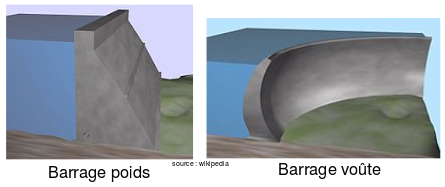
\includegraphics[scale=0.5]{barrages.png}
\caption{Barrages}
\label{fig:barrages}
\end{figure}

Lors de la construction d'un barrage, il faut étudier la géologie du milieu. Si le sol n'est pas adapté, la barrage pourrait céder.

\section{Microcentrales électriques}
Celles-ci sont implémentées le long d'un cours d'eau et reproduisent l'énergie potentielle d'une chute d'eau en canalisant une partie d'un cours d'eau. Celles-ci sont composées de (figure~\ref{fig:microcentrale}): 
\begin{itemize}
\item Un barrage (optionnel), permettant de créer un seuil, une prise d'eau
\item Une prise d'eau
\item Un canal de dérivation (ou conduite forcée), qui amène l'eau jusqu'à la centrale permettant de reproduire artificiellement une chute d'eau.
\item Une centrale hydroélectrique
\item Une échelle à poissons (optionnel)
\end{itemize}

\begin{figure}[ht!]
\centering
\includegraphics[scale=0.5]{microcentrale.png}
\caption{Microcentrale}
\label{fig:microcentrale}
\end{figure}

Il existe plusieurs types de centrales selon le type de cours d'eau et la puissance désirée : 
\begin{itemize}
\item Petite centrale : 2-\unit{10}{\mega\watt}
\item Mini-centrale : 0.5-\unit{2}{\mega\watt}
\item Micro-centrale : 0.02-\unit{0.5}{\mega\watt}
\item Pico-centrale : <\unit{0.02}{\mega\watt}
\end{itemize}

Ces stations n'influent pas le niveau et le débit de l'eau et ont un faible impact environnemental.

\section{Géothermie}
L'énergie géothermique est associée à la chaleur du sol, dans lequel les températures sont basses (<\unit{30}{\celsius}) ou hautes (>\unit{90}{\celsius}) selon la profondeur. Les hautes températures proviennent  principalement de la radioactivité naturelle des couches terrestres. La température moyenne du sol à 1 mètre de profondeur est de 8-\unit{1}{\celsius}.

Les avantages de la géothermies sont : 
\begin{itemize}
\item Très peu d'émission de gaz à effet de serre, énergie directement utilisable.
\item Constance dans la production, la température du sol est relativement constante à partir d'une ceraitne profondeur.
\item Production locale, possibilité d'installations de petites tailles, impact visuel limité.
\item Potentiel quasi illimité.
\end{itemize}

\subsection{Classification de l'énergie géothermique}
On peut classer la géothermie fonction de la température d'utilisation :
\begin{itemize}
\item Haute et moyenne énergie : >\unit{90}{\celsius}, production d'électricité.
\item Basse température : entre 30 et \unit{90}{\celsius}, production de chaleur.
\item Très basse température : <\unit{30}{\celsius}, pompes à chaleur géothermiques.
\end{itemize}
La température du sous-sol augmente avec la profondeur selon un gradient géothermique (presque linéaire), le flux thermique peut donc être évalué comme : $Q = k \Delta T$

\subsection{Caractéristiques thermiques des sols}
Les paramètres caractéristiques sont : la conuctivité thermique [\unit{\watt\per\meter\usk\kelvin}], la capacité thermique [\unit{\joule\per\cubic\meter\usk\kelvin}] et la diffusivité thermique [\unit{\meter\squared\per\second}]. Ces paramètres sont fonctions de l'humidité et de la composition du sol. 

Les sols sont des mauvais conducteurs de chaleur mais d'assez bons accumulateurs de chaleur. La présence d'une nappe améliore la conductivité thermique ainsi que la capacité thermique du terrain.
\bigbreak
La quantité de chaleur pouvant être extraite du sol dépend de plusieurs paramètres et doit être prise en compte pour le dimensionnement du système géothermique :
\begin{itemize}
\item (Hydro-)géologie du terrain : nature et épaisseurs des différentes couches, perméabilité,...
\item Température du sous-sol.
\item Transfert annuel net d'énergie au sous-sol.
\item Caractéristiques du fluide géothermal.
\item Caractéristiques des terrains exploités.
\item Caractéristiques du matériel géothermique utilisé.
\end{itemize}
\bigbreak

La température du sol suit une loi sinusoïdale (figure~\ref{fig:geotemp}) et les variations quotidiennes sont imperceptibles à 1 mètre de profondeur tandis que les variations saisonnières s'atténuent à 10 mètre de profondeur.
\begin{figure}[ht!]
\centering
\includegraphics[scale=0.65]{geo_temp.png}
\caption{Variations de température du sol}
\label{fig:geotemp}
\end{figure}

\subsection{Installation très basse énergie}

Il est possible d'utiliser soit l'eau (nappes phréatiques ou eau de surface) soit le sol comme énergie géothermique.

Un système géothermique peut être soit ouvert soit fermé. Un système fermé fait circuler un fluide dans le sol et récupère la chaleur du sol par convection. Dans un système ouvert, le fluide (eau) est injecté dans le sol puis extrait en continu. Les différents composants d'une système géothermique sont : un capteur géothermique qui capte la chaleur du sol, un générateur thermodynamique qui transforme les calories issues du captage en énergie calorifique et un circuit de distribution de chaleur (radiateurs,...).

Il existe plusieurs types d'installations. Tout d'abord, l'installation horizontale, qui constiste en un réseau de tuyaux enterrés entre 60 et \unit{120}{\centi\meter} de profondeur dans lesquels circulent un fluide caloporteur. C'est la méthode la plus répandue, elle est adaptée aux maisons individuelles, plus particulièrement aux maisons neuves.

Une autre méthode est de mettre le réseau de tubes vertical, et aller chercher la chaleur plus profond dans le sol.

Enfin, il existe des pieux géothermiques qui s'intègrent dans la structure de l'ouvrage. Des échangeurs de chaleur sont donc intégrés  dans les fondations.


\end{document}